\documentclass[a4paper,oneside,11pt]{report}
\usepackage{myStyle}

% --- Additions for this report (the template's myStyle.sty is unchanged) ---
\usepackage{booktabs}
\usepackage{longtable}
\usepackage{tabularx}
\usepackage{listings}
\usepackage{amsmath}
\usetikzlibrary{positioning,shapes.geometric,arrows.meta,fit,calc}
\captionsetup{labelfont=bf,font=small}
\lstset{basicstyle=\ttfamily\small,backgroundcolor=\color{gray!8},frame=single,
        rulecolor=\color{gray!40},columns=fullflexible,breaklines=true,
        aboveskip=8pt,belowskip=4pt,showstringspaces=false}
\renewcommand{\lstlistlistingname}{Listings}
\usepackage[hidelinks]{hyperref}
\setlength{\emergencystretch}{3em} % lets lines with long code names wrap instead of overflowing
\usepackage{placeins} % \FloatBarrier keeps each walkthrough section's pictures inside it
\usepackage{needspace}
% Let pages hold several figures (the screenshot rows) instead of leaving gaps
\renewcommand{\topfraction}{0.9}\renewcommand{\bottomfraction}{0.8}
\renewcommand{\textfraction}{0.07}\renewcommand{\floatpagefraction}{0.75}
\setcounter{topnumber}{3}\setcounter{bottomnumber}{2}\setcounter{totalnumber}{4}
% Tables are single-spaced (body text keeps the template's 1.5 spacing)
\usepackage{etoolbox}
\AtBeginEnvironment{table}{\renewcommand{\baselinestretch}{1.0}\selectfont}
\AtBeginEnvironment{longtable}{\renewcommand{\baselinestretch}{1.0}\selectfont}
% Screenshot frames in Chapter 7 (tex/walkthrough.tex is generated by make_walkthrough.py)
\setlength{\fboxrule}{0.3pt}

% Edit these in one place
\newcommand{\projecttitle}{Sarabo: An Electronics Repair Service Management Platform}
\newcommand{\studentname}{Jahid Hasan}
\newcommand{\studentid}{222-115-116}
\newcommand{\studentbatch}{57 (C)}
\newcommand{\supervisorname}{Shrabanti Chowdhury}
\newcommand{\supervisordesig}{Senior Lecturer}
\newcommand{\reviewerone}{Nabila Zannat Rifa}
\newcommand{\reviewertwo}{Md. Fahmidur Rahman Sakib}
\newcommand{\submissiondate}{26 October 2026}
% Verified test results (see Chapter 9)
\newcommand{\servertestcount}{2,761}
\newcommand{\clienttestcount}{58}

% TikZ styles shared by every diagram
\tikzset{
  box/.style={draw,rounded corners=2pt,fill=gray!6,align=center,font=\small,minimum height=8mm,inner sep=4pt},
  hl/.style={box,fill=blue!6},
  dec/.style={draw,diamond,aspect=2.2,fill=yellow!10,align=center,font=\small,inner sep=1pt},
  db/.style={draw,cylinder,shape border rotate=90,aspect=0.25,fill=green!6,align=center,font=\small,minimum height=10mm},
  arr/.style={-{Stealth[length=2mm]},thick},
  lbl/.style={font=\scriptsize,fill=white,inner sep=1pt}
}

\begin{document}
\pagenumbering{Alph}
\pagestyle{empty}
% --- PAGE 1: MAIN TITLE PAGE ---
\begin{titlepage}
\begin{center}
    \begin{figure}[h]
        \centering
        
\includegraphics[scale=0.2]{./img/metrologo}
    \end{figure}
    \vfill
    {\huge \textbf{A Project Report}} \\
    \vspace{1cm}
    {\Large Submitted To} \\
    \vspace{0.5cm}
    {\large The Department of Computer Science and Engineering, Metropolitan University, in partial fulfillment of the requirements for the degree of Bachelor of Science in Computer Science and Engineering.} \\
    \vfill
    {\Large On} \\
    {\LARGE \textbf{\projecttitle}} \\
    \vfill
    {\Large Submitted By} \\
    \vspace{0.5cm}
    \textbf{\studentname} \\
    ID No: \studentid \\
    Batch: \studentbatch
    \vfill
    {\Large Under The Supervision of} \\
    \textbf{\supervisorname} \\
    \supervisordesig \\
    Department of Computer Science and Engineering\\
    Metropolitan University, Sylhet \\
    \vfill
    \textbf{Submission Date: \submissiondate}
\end{center}
\end{titlepage}

% --- PAGE 2: STUDENT'S DECLARATION ---
\newpage
\begin{center}
    \begin{figure}[h]
        \centering
        
\includegraphics[scale=0.2]{./img/metrologo}
    \end{figure}
    \vspace{1cm}
    {\Large \textbf{STUDENT'S DECLARATION}}
\end{center}
\vspace{1cm}
\noindent I, the undersigned, solemnly declare that the project report entitled \textbf{``\projecttitle''} is based on my original project work carried out during the course of study under the supervision of \textbf{\supervisorname}. The analysis, design, implementation, testing, and documentation presented in this report were completed as an individual final year project, except where the work of others has been properly cited.

\vspace{0.5cm}
\noindent I further declare that, to the best of my knowledge and belief, this report has not been submitted elsewhere in substantially the same form for the requirement of any other degree. All external literature, standards, documentation, libraries, and technologies used in the project have been acknowledged in the reference section.

\vspace{3cm}
\noindent \rule{6cm}{0.4pt} \\
\textbf{\studentname} \\
ID No: \studentid \\
Batch: \studentbatch

% --- PAGE 3: SUPERVISOR'S RECOMMENDATION ---
\newpage
\begin{center}
    \begin{figure}[h]
        \centering
        
\includegraphics[scale=0.2]{./img/metrologo}
    \end{figure}
    \vspace{1cm}
    {\Large \textbf{SUPERVISOR'S RECOMMENDATION}}
\end{center}
\vspace{1cm}
\noindent The project work entitled \textbf{``\projecttitle''} submitted by \textbf{\studentname}, ID No: \studentid, Batch: \studentbatch, is a record of project work carried out under my supervision. I hereby recommend that this project report is satisfactory in partial fulfillment of the requirements for the degree of Bachelor of Science in Computer Science and Engineering and may be processed for further evaluation.

\vspace{3cm}
\noindent \rule{7cm}{0.4pt} \\
\textbf{\supervisorname} \\
\supervisordesig \\
Department of Computer Science and Engineering\\
Metropolitan University, Sylhet \\
(Supervisor)

% --- PAGE 4: LETTER OF APPROVAL ---
\newpage
\begin{center}
    \begin{figure}[h]
        \centering
        
\includegraphics[scale=0.2]{./img/metrologo}
    \end{figure}
    \vspace{1cm}
    {\Large \textbf{LETTER OF APPROVAL}}
\end{center}
\vspace{1cm}
\noindent This is to certify that the project work entitled \textbf{``\projecttitle''} submitted by \textbf{\studentname}, ID No: \studentid, Batch: \studentbatch, has been studied and approved by the project examination committee as satisfactory in partial fulfillment of the requirements for the degree of Bachelor of Science in Computer Science and Engineering.

\vspace{2.5cm}

\noindent \rule{6cm}{0.4pt} \\
\textbf{\supervisorname} \\
\supervisordesig, Department of Computer Science and Engineering \\
Supervisor

\vspace{2cm}

\noindent
\begin{tabular}{@{}p{0.48\textwidth} p{0.48\textwidth}@{}}
    \rule{6cm}{0.4pt} & \rule{6cm}{0.4pt} \\
    \textbf{\reviewerone} & \textbf{\reviewertwo} \\
    Senior Lecturer & Senior Lecturer \\
    Reviewer 1 & Reviewer 2
\end{tabular}

\pagestyle{plain}
\clearpage\pagenumbering{Roman}
\addcontentsline{toc}{section}{Abstract}
\documentclass{standalone}
\usepackage{standalone}

\begin{document}
\chapter*{Abstract}
Electronics repair in Bangladesh is still largely informal: customers hand over a phone, laptop or appliance without knowing the final price, cannot see where it is, and have little recourse if something goes wrong, while technicians have no structured way to find nearby work or get paid reliably. This project presents \textbf{Sarabo}, a web-based electronics repair service management platform that turns this process into a tracked, priced and auditable service.

Sarabo connects three roles. A \emph{Customer} describes the problem (optionally letting AI fill the form from Bangla, English or Banglish text and a damage photo), books a pickup window, compares offers from qualified technicians in the same region, pays an inspection fee that counts toward the final price, approves or rejects the itemised quote, pays, tracks progress and reviews the technician. A \emph{Technician} finds work on an open jobs board, sends offers guided by a data-driven price guide, inspects, quotes, repairs and withdraws earnings through bKash. An \emph{Admin} approves technicians, maintains a versioned catalogue of 45 services, handles missed pickups and refunds, moderates reviews and reads reports with an AI-written summary.

The client uses React 19 and Vite; the server uses Node.js, Express 5 and MongoDB, with Firebase Authentication, Stripe payments and refunds, private Supabase storage and Google Gemini. Every money- or assignment-changing step runs in a database transaction, Stripe's signed webhook is the single source of payment truth, and a 90/10 technician/platform settlement is frozen at payment time. The system is deployed on Vercel and Firebase Hosting and was verified with \servertestcount{} passing automated server checks, \clienttestcount{} passing browser tests, lint and build checks, and continuous integration.

\paragraph*{Keywords:} Electronics repair, service marketplace, workflow management, React, Express, MongoDB, Stripe, role-based access control, generative AI.
\end{document}

\clearpage
\addcontentsline{toc}{section}{Acknowledgements}
\documentclass{standalone}
\usepackage{standalone}

\begin{document}
\chapter*{Acknowledgements}
First, I would like to thank my supervisor, \textbf{\supervisorname}, \supervisordesig, Department of Computer Science and Engineering, Metropolitan University, for her guidance, feedback and encouragement throughout this final year project. Her advice helped me turn Sarabo from a rough application idea into a properly structured service management platform.

I am also thankful to the faculty members of the Department of Computer Science and Engineering for the academic foundation this work stands on, and to my reviewers, \textbf{\reviewerone} and \textbf{\reviewertwo}, for evaluating the project and sharing their feedback.

Finally, I owe a great deal to the open-source communities and documentation writers behind React, Express, MongoDB, Firebase, Stripe, Supabase, Google Gemini, TanStack Query, Tailwind CSS, Playwright and the other tools Sarabo uses. Without their work, building and testing a full-stack platform of this size on my own would not have been possible.
\end{document}

\clearpage
\addcontentsline{toc}{section}{Table of Contents}
\setcounter{tocdepth}{1} % chapters and sections only, keeps the contents list short
% The lists use single line spacing; the chapters keep the template's 1.5 spacing.
{\renewcommand{\baselinestretch}{1.0}\selectfont
\tableofcontents
\clearpage
\addcontentsline{toc}{section}{\listtablename}
\listoftables
\clearpage
\addcontentsline{toc}{section}{\listfigurename}
\listoffigures
\addcontentsline{toc}{section}{Listings}
\lstlistoflistings
}
\clearpage\pagenumbering{arabic}

\documentclass{standalone}
\usepackage{standalone}

\begin{document}
\chapter{Introduction}

\section{Project Overview}
Sarabo is a web-based platform for managing electronics repair services, which I developed on my own as my final year project. It handles the whole life of a repair request, from the moment a customer describes a faulty device to the moment the technician gets paid, as one workflow that can be traced from start to finish. Three people are involved: a \emph{Customer} who needs something repaired, a \emph{Technician} who does the repair, and an \emph{Admin} who keeps the service running.

The most important design decision was to treat a repair request as a \emph{case that moves through states}, not as a simple database record. Every important activity moves the case from one clearly defined state to the next: creating the request, technician offers, booking, pickup, inspection, quotation, payment, repair, hand-over, settlement and feedback. For each move, the server checks that this user is allowed to make it at this moment. This is the main difference between Sarabo and a basic create-read-update-delete (CRUD) application. Whether a later action is correct depends on earlier actions having happened, and on them having happened only once.

The project was built in two main stages. In the first stage (July--August 2026) I built the core repair lifecycle, in which an admin assigned a technician to each request. An earlier version of this report described that stage. In the second stage (September--October 2026) Sarabo became a two-sided marketplace. It gained an open jobs board where technicians send offers, a paid inspection fee with automatic refunds, pickup scheduling, customer reviews, email notifications, operational reports, four AI-assisted features and a production deployment. A final phase (11--16 October 2026) then added offer ranking, a repair warranty, deadlines for every waiting state, a minimum inspection fee and faster hosting. This report describes the system as it stands after all of that work.

\section{Problem Statement}
A repair service needs both technical work and a lot of coordination. The customer has to describe the device and the problem, get an idea of the cost before handing the device over, choose someone they can trust, pay safely and find out whether the device has actually been repaired. The technician needs a steady supply of nearby jobs that match their skills, a clear way to record an inspection and a quote, and a reliable way to be paid. The administrator needs to see which requests are stuck, which payments need attention, and whether customers are being turned away.

When all of this is handled through phone calls, messaging apps and paper notes, things easily go wrong. A customer is charged before agreeing to a price. A technician is booked twice for the same time. An inspection fee is neither refunded nor taken off the bill. A technician's earning is paid out twice, or private photos of a customer's device end up in the wrong hands. Sarabo deals with this by modelling the repair process as a workflow that knows each user's role, with clear rules for every change of state, validation on the server and updates that run as transactions.

\section{Motivation}
I had five main reasons for choosing this project:
\begin{enumerate}
  \item to work on a real, local problem, by making electronics repair in Bangladesh more transparent and trustworthy for customers and easier to access for independent technicians;
  \item to build a realistic full-stack system that goes beyond simple CRUD, where roles and state changes are enforced on the server instead of being left to the browser;
  \item to integrate real, production-grade services (identity, card payments and refunds, private file storage, email and generative AI) without exposing any privileged credentials;
  \item to use generative AI where it actually helps people, while keeping it safe: it must not invent prices or leak personal data, and its usage must have hard limits; and
  \item to give every user a clear interface in which the next useful action is always easy to see.
\end{enumerate}

\section{Objectives}
The main objective was to build a reliable platform that manages the complete lifecycle of an electronics repair. Table~\ref{tab:objectives} lists the specific objectives.

\begin{table}[htbp]
\centering
\caption{Project objectives}
\label{tab:objectives}
\begin{tabularx}{\textwidth}{@{}lX@{}}
\toprule
\textbf{No.} & \textbf{Objective} \\
\midrule
O1 & Provide secure authentication and role-aware access for Customer, Technician and Admin. \\
O2 & Let customers create structured repair requests (device, service, region, pickup window, optional damage photos), with optional AI assistance. \\
O3 & Match requests only to approved technicians with the right expertise in the customer's region, through an open offer-based job portal. \\
O4 & Support a paid inspection fee that books a technician, is credited toward the final price, and is refunded or split fairly when the repair does not go ahead. \\
O5 & Provide an inspection and quotation workflow with customer approval, rejection and revision. \\
O6 & Accept payment only for approved amounts, with a single authoritative paid state and downloadable receipts. \\
O7 & Support repair progress, completion evidence, receipt confirmation and customer feedback. \\
O8 & Keep customers and technicians informed through in-app notifications, email, reminders and a sanitized public tracking page. \\
O9 & Provide a technician wallet with a 90/10 settlement and controlled bKash withdrawals. \\
O10 & Give admins operational oversight: attention lists, reports, catalogue management and moderation. \\
O11 & Validate the system through automated server tests, browser tests, static checks and continuous integration, and deploy it. \\
O12 & Protect customers after the repair with a warranty, and make sure no request can get stuck in any state. \\
\bottomrule
\end{tabularx}
\end{table}

\section{Scope}
The finished system covers the following: registration and email verification, technician applications with structured expertise, a versioned service catalogue, AI-assisted request creation, damage-photo upload and pickup scheduling. It also covers an open jobs board with offers, booking with an inspection fee and refunds, inspection, quotation and revision, Stripe payment, repair progress with completion evidence, receipt confirmation, and reviews and private reports. On top of that there are in-app and email notifications, public tracking, a technician wallet with bKash withdrawals, an AI customer-support chat, admin reports with an AI summary, offer ranking, a 30-day repair warranty, deadlines and admin alerts for stalled work, a record of the device's condition at pickup, and a production deployment.

The project does not try to do everything a commercial field-service company would. Automatic mobile-wallet payouts, cash payment, spare-parts inventory, live GPS tracking of technicians, native mobile apps and accounting for several branches are outside the current scope. Chapter~\ref{ch:limitations} discusses them as future work.

\section{Individual Contribution}
Sarabo is a solo project, and I, \studentname, did all of the work on it. This covered requirements analysis, data modelling, user-interface design, frontend and backend development, the workflow and financial logic, integration of the external services, AI prompt and safety design, testing, deployment, debugging and writing this report.

\section{Report Organization}
Chapter~2 gives the technical background and looks at related systems. Chapter~3 sets out the stakeholders and requirements. Chapter~4 presents the architecture, the data model and the state model. Chapter~5 describes the implementation and how development was carried out. Chapter~6 explains the core workflows and business rules. Chapter~7 walks through the running system, with screenshots of every main step for each role. Chapter~8 covers the AI-assisted features and how they are kept safe. Chapter~9 discusses security, reliability and data integrity, and Chapter~10 presents testing and evaluation. Chapter~11 lists limitations and future work, and Chapter~12 concludes the report. The appendices summarise the API, the data model and the financial rules, give build notes, and record one notable incident from development.

\end{document}
  % Chapter 1 Introduction
\documentclass{standalone}
\usepackage{standalone}

\begin{document}
\chapter{Background and Related Work}

\section{Web-Based Service Management}
A service management platform differs from a static information system because each request evolves through a sequence of operational decisions made by different people. Sarabo follows a resource-oriented HTTP API design influenced by the REST architectural style~\cite{fielding2000}. The browser presents the workflow, but the server remains the only authority on whether a transition is legal.

\section{Single-Page Application Architecture}
The client is a React single-page application. React provides a component model for composing stateful interfaces~\cite{react}, React Router maps public pages and role-specific dashboard routes, and TanStack Query manages asynchronous server state, caching and invalidation~\cite{tanstack}. This separation matters in Sarabo because server data such as request status, offers, quotations, wallet balances and notifications can change independently of the form a user is filling in. Vite~\cite{vite} provides the development server and production bundling, and Tailwind CSS~\cite{tailwind} the styling system.

\section{RESTful API and Express}
The server uses Express~5~\cite{express} as its HTTP framework. Routes are grouped by domain (users, technicians, repair requests, job applications, inspections, quotations, payments, repairs, wallet, feedback, notifications, tracking, service definitions, damage uploads, support and administration). Sensitive routes apply authentication middleware and role checks before any database operation.

\section{Document Database and Transactions}
MongoDB is the primary database~\cite{mongodb}. A document model suits a repair request: it has a stable identity but accumulates nested workflow information (product snapshot, service and price snapshot, damage images, inspection, quote and quote history, payments, repair evidence, assignment history and settlement). Separate collections are used where an independent lifecycle, index or audit trail is needed, such as job applications, payments, notifications, tracking events, withdrawals and reviews. MongoDB multi-document transactions, available on replica sets, let several of these collections change together or not at all.

\section{Authentication and Authorization}
Firebase Authentication supplies user identity and signed ID tokens~\cite{firebaseauth}. The client attaches the token to every protected API request, and the server verifies it with the Firebase Admin SDK before trusting the caller's email. Authorization is then role-based (Customer, Technician, Admin) and state-based (the request must be in the right stage). For backward compatibility the stored role value for Technician remains \texttt{rider}, inherited from the original codebase, while every user-facing label says ``Technician''.

\section{Online Payment Processing}
Sarabo uses Stripe Checkout for card payments~\cite{stripe}. The design treats the server-side record of payment as authoritative: Stripe calls a webhook whose signature is verified against a shared secret~\cite{stripewebhooks}, so the payment is recorded even if the customer closes the browser before returning to the success page. Refunds are requested through Stripe's API with idempotency keys so they cannot be issued twice. All payments currently run in Stripe test mode.

\section{Private Object Storage}
Damage and repair-evidence images are stored in a private Supabase Storage bucket~\cite{supabase}. The server issues short-lived signed URLs: the browser uploads bytes directly to storage, the server then verifies the stored object's real type and size, and every later view uses a fresh signed read URL. Large files never pass through the API server, and the privileged storage key never reaches the browser.

\section{Large Language Models in Applications}
Large language models (LLMs) such as Google Gemini~\cite{gemini} can turn free text into structured data, summarise information and draft natural-language messages. They can also produce confident but wrong output (``hallucination''), be manipulated by instructions hidden in user text (prompt injection), and generate unpredictable cost. OWASP lists prompt injection and overreliance among the main risks of LLM applications~\cite{owaspllm}. Sarabo therefore uses AI only as an \emph{assistant}: the model's answer is constrained to a JSON schema, validated against live data on the server, never allowed to set a price, and always reviewed by a human before it takes effect (Chapter~\ref{ch:ai}).

\section{Usability and Accessibility}
The interface follows an action-first approach: the current stage of a repair and the next action for the signed-in role get more visual weight than secondary data. A recurring ``service spine'' (Request, Inspect, Approve, Repaired) appears on the home page, the public tracking page and every dashboard. Labels, focus order, keyboard access, colour contrast, reduced motion and responsive layouts from 320\,px upward follow the WCAG~2.2 guidance~\cite{wcag22}.

\section{Related Systems}
Repair and home-service needs in Bangladesh are served today in three broad ways:
\begin{itemize}
  \item \textbf{Local repair shops and freelance technicians}, found through word of mouth or social media. Prices are negotiated in person, there is no tracking and little recourse.
  \item \textbf{Brand service centres}, which offer reliable repair for their own products but cover only one brand and are concentrated in large cities.
  \item \textbf{General on-demand service marketplaces} such as Sheba.xyz in Bangladesh~\cite{sheba} and Urban Company in South Asia~\cite{urbancompany}, which let customers book many kinds of household services from listed providers.
\end{itemize}

International platforms such as Thumbtack~\cite{thumbtack} popularised the model in which customers describe a job and several professionals respond with quotes. Sarabo adopts this offer model but specialises it for electronics repair, where the true price is usually unknown until the device has been opened. Table~\ref{tab:related} compares the approaches on the features most relevant to this project.

\begin{table}[htbp]
\centering
\caption{Comparison of approaches to electronics repair}
\label{tab:related}
\small
\begin{tabularx}{\textwidth}{@{}Xccc@{}}
\toprule
\textbf{Capability} & \textbf{Local shop} & \textbf{General marketplace} & \textbf{Sarabo} \\
\midrule
Online request with device and problem details & -- & \checkmark & \checkmark \\
Price estimate before hand-over & -- & Partial & \checkmark \\
Several competing offers per job & -- & Varies & \checkmark \\
Separate inspection fee credited to final price & -- & -- & \checkmark \\
Formal inspection and itemised quote & -- & Varies & \checkmark \\
Online payment with receipt & -- & \checkmark & \checkmark \\
Step-by-step public tracking & -- & Partial & \checkmark \\
Technician matched by repair-specific expertise & -- & Partial & \checkmark \\
Bangla/Banglish AI request assistance & -- & -- & \checkmark \\
\bottomrule
\end{tabularx}
\end{table}

Sarabo's contribution is not a new algorithm. Its engineering value lies in combining patterns from ticketing systems (a trackable case with an identifier and history), field-service systems (assignment, inspection, completion), marketplaces (offers, payment, commission, payouts) and evidence-driven workflows (private photos and completion records) into one coherent repair workflow with explicit state, money and authorization rules.

\end{document}
      % Chapter 2 Background and Related Work
\documentclass{standalone}
\usepackage{standalone}

\begin{document}
\chapter{Requirements Analysis}

\section{Stakeholders and Roles}
Sarabo has three roles for signed-in users, plus visitors who use it without an account. Table~\ref{tab:roles} summarises what each of them wants from the system.

\begin{table}[htbp]
\centering
\caption{User roles}
\label{tab:roles}
\small
\begin{tabularx}{\textwidth}{@{}p{2.2cm}p{3.6cm}X@{}}
\toprule
\textbf{Role} & \textbf{Primary goal} & \textbf{Representative actions} \\
\midrule
Customer & Get a device repaired at a fair, known price & Create request (optionally with AI help), add photos, pick a pickup slot, compare offers, pay inspection fee, approve or reject quote, pay, track, confirm receipt, review or report the technician, claim warranty \\
Technician & Find suitable work and get paid & Apply with expertise and region, browse the jobs board, send offers, inspect, quote, revise, repair, complete, view wallet, withdraw via bKash \\
Admin & Keep the service healthy & Approve technicians, edit catalogue and prices, handle missed pickups, refunds, disputes and warranty reviews, process withdrawals, moderate reviews and reports, read reports \\
Visitor & Learn about the service & Browse services, service areas and open jobs, track a repair with a tracking code, ask the AI support chat \\
\bottomrule
\end{tabularx}
\end{table}

\section{Functional Requirements}
Table~\ref{tab:fr} lists the functional requirements. FR-21 to FR-32 were added during the second development stage, and FR-33 to FR-38 during the final phase.

\begin{longtable}{@{}p{1.4cm}p{13cm}@{}}
\caption{Functional requirements}\label{tab:fr}\\
\toprule
\textbf{ID} & \textbf{Requirement} \\
\midrule
\endfirsthead
\toprule
\textbf{ID} & \textbf{Requirement} \\
\midrule
\endhead
\bottomrule
\endfoot
FR-01 & The system shall authenticate users (email/password and Google) and protect private routes. \\
FR-02 & The system shall distinguish Customer, Technician and Admin capabilities on the server. \\
FR-03 & A verified Customer shall be able to create a structured repair request for a catalogue service. \\
FR-04 & The service catalogue shall provide active device and repair categories with BDT estimate ranges, inspection fee caps (never below the minimum fee) and required expertise level. \\
FR-05 & Customers shall be able to attach up to three damage photos through a controlled private-storage workflow. \\
FR-06 & Users shall be able to apply as Technicians with region, district and structured expertise; Admin shall approve or reject applications. \\
FR-07 & The assigned Technician shall submit an inspection before a quote can be submitted. \\
FR-08 & The Technician shall submit an itemised quote (labour, parts, additional charges). \\
FR-09 & The Customer shall approve or reject the quote; after rejection the Technician may revise once more or close the request. \\
FR-10 & Payment shall be possible only for an approved quote and never twice. \\
FR-11 & The Technician shall record repair progress and completion with optional evidence photos. \\
FR-12 & The Customer shall confirm receipt of the repaired device. \\
FR-13 & The system shall send role-appropriate in-app notifications for workflow events. \\
FR-14 & A public tracking page shall show a sanitized timeline by tracking code, without personal or payment data. \\
FR-15 & A 90/10 Technician/platform settlement shall be frozen when the repair is paid. \\
FR-16 & Technicians shall request withdrawals up to their server-computed available balance; Admin shall mark each as paid (with bKash TrxID) or rejected exactly once. \\
FR-17 & A customer shall be able to cancel a request before a technician is booked. \\
FR-18 & Admin shall be able to edit the service catalogue; price changes shall create a new version without changing existing requests. \\
FR-19 & Technicians shall be able to edit their expertise; Admin shall see technician availability. \\
FR-20 & Customers shall be able to download a PDF receipt for every payment. \\
FR-21 & A request shall be accepted only if at least one approved Technician in the customer's region can perform it; refused demand shall be counted. \\
FR-22 & Customers shall choose a two-hour pickup slot (Saturday--Thursday, up to 7 days ahead) subject to per-region capacity, and may reschedule before pickup. \\
FR-23 & Open requests shall appear on a public jobs board; matching Technicians shall be notified and may send offers (estimate range, inspection fee, note). \\
FR-24 & The Customer shall compare offers and choose one, or reject one (the job is reposted and the Technician may send one revised offer). \\
FR-25 & Choosing an offer with a fee shall open a Stripe payment; the confirmed payment shall book the Technician atomically. \\
FR-26 & The inspection fee shall be credited toward the final quote, refunded when the visit fails or is cancelled in time, and split 90/10 when kept. \\
FR-27 & Customers shall rate a completed repair (1--5 with optional comment) or file a private report; Admin shall moderate both. \\
FR-28 & The system shall email request confirmations, pickup reminders and new-job alerts, and post in-app pickup reminders daily. \\
FR-29 & Admin shall see an attention list (overdue and missed pickups, unmatchable requests, no offers in 24 hours, refunds waiting) and period reports. \\
FR-30 & An AI helper shall turn a free-text description and/or damage photo into a draft request that the customer reviews. \\
FR-31 & Technicians shall see a price guide from past offers and may ask AI to draft their offer note. \\
FR-32 & An AI support chat shall answer visitor questions from live catalogue data, and Admin reports shall include an AI summary checked against the real figures. \\
FR-33 & Offers shall be ranked by rating, reliability, price, district and reply time, with the best match and its reasons shown; the customer still chooses. \\
FR-34 & A finished repair shall carry a 30-day warranty: free re-inspection by the same technician, free re-repair if covered, and an admin refund if it cannot be fixed. \\
FR-35 & Every waiting state shall have a deadline, an automatic step or an admin alert (unpaid quote, not repairable, repair that cannot be finished, receipt not confirmed, device not returned, stalled work). \\
FR-36 & The technician shall record the device's condition and accessories at pickup, and may report a customer who is not home without it counting as a no-show. \\
FR-37 & Every repair shall have an inspection fee of at least 100 BDT (200 BDT when the estimate exceeds 1,000 BDT). \\
FR-38 & Technicians shall edit their own name, phone, address and service area (the area only while no repair is active). \\
\end{longtable}

\section{Non-Functional Requirements}
\begin{table}[htbp]
\centering
\caption{Non-functional requirements}
\label{tab:nfr}
\small
\begin{tabularx}{\textwidth}{@{}p{2.6cm}X@{}}
\toprule
\textbf{Category} & \textbf{Requirement} \\
\midrule
Security & Identity, role, prices, fees, balances and refund decisions are derived or validated on the server. Private images are reachable only through short-lived signed URLs. Secrets never reach the browser. \\
Consistency & Steps that change several records (booking, approval, completion, settlement, refunds) run as database transactions. \\
Reliability & Repeated or concurrent actions return controlled conflicts instead of repeating money or state changes. Failed refunds stay pending and can be retried. Email or notification failures never fail the main action. \\
Privacy & Public pages (tracking, jobs board) expose no names, emails, addresses or payment data. AI providers receive no personal identifiers. \\
Cost control & Every AI feature has per-user and site-wide daily limits stored in the database, and is off unless explicitly enabled. \\
Usability & Each screen shows the current stage and the next action for that role; empty, loading and error states are truthful. \\
Accessibility & Keyboard access, visible focus, sufficient contrast, labelled controls, reduced-motion support, layouts from 320\,px. \\
Performance & Cached server state on the client, code-split routes, direct-to-storage uploads, paginated lists. \\
Maintainability & Workflow rules, status presentation and query keys are centralised; CI runs lint, build and tests on every push. \\
Auditability & Tracking events, assignment history, quote history, payment rows, refund state, withdrawal processing and moderation history are kept. \\
\bottomrule
\end{tabularx}
\end{table}

\section{Service Catalogue}
The catalogue has \textbf{45 services} spread over eight device categories (Table~\ref{tab:catalogue}). Each service links a device category to a repair category. It also has an estimated price range in BDT, a maximum inspection fee, the expertise level a technician needs (beginner, intermediate, advanced or expert) and an estimated duration. These prices are only estimates. The amount the customer actually pays is always the technician's written quote after inspection.

\begin{table}[htbp]
\centering
\caption{Service catalogue summary with sample services}
\label{tab:catalogue}
\small
\begin{tabularx}{\textwidth}{@{}p{2.8cm}cXr@{}}
\toprule
\textbf{Device} & \textbf{Services} & \textbf{Sample service} & \textbf{Estimate (BDT)} \\
\midrule
Smartphone & 8 & Screen Replacement & 1,500--6,000 \\
Laptop / Computer & 8 & Motherboard Repair & 2,500--12,000 \\
Television & 5 & Screen / Panel Repair & 4,000--18,000 \\
Refrigerator & 6 & Compressor / Refrigerant Service & 3,500--15,000 \\
Washing Machine & 6 & Control Board Repair & 2,000--7,000 \\
Air Conditioner & 6 & Gas Refill / Compressor Repair & 3,000--20,000 \\
Microwave Oven & 4 & Electrical / Power Repair & 1,500--5,000 \\
Other Electronics & 2 & General Repair & 1,000--5,000 \\
\midrule
\textbf{Total} & \textbf{45} & & \\
\bottomrule
\end{tabularx}
\end{table}

\section{Use-Case View}
Figure~\ref{fig:usecase} shows the main things each role does on the platform.

\begin{figure}[htbp]
\centering
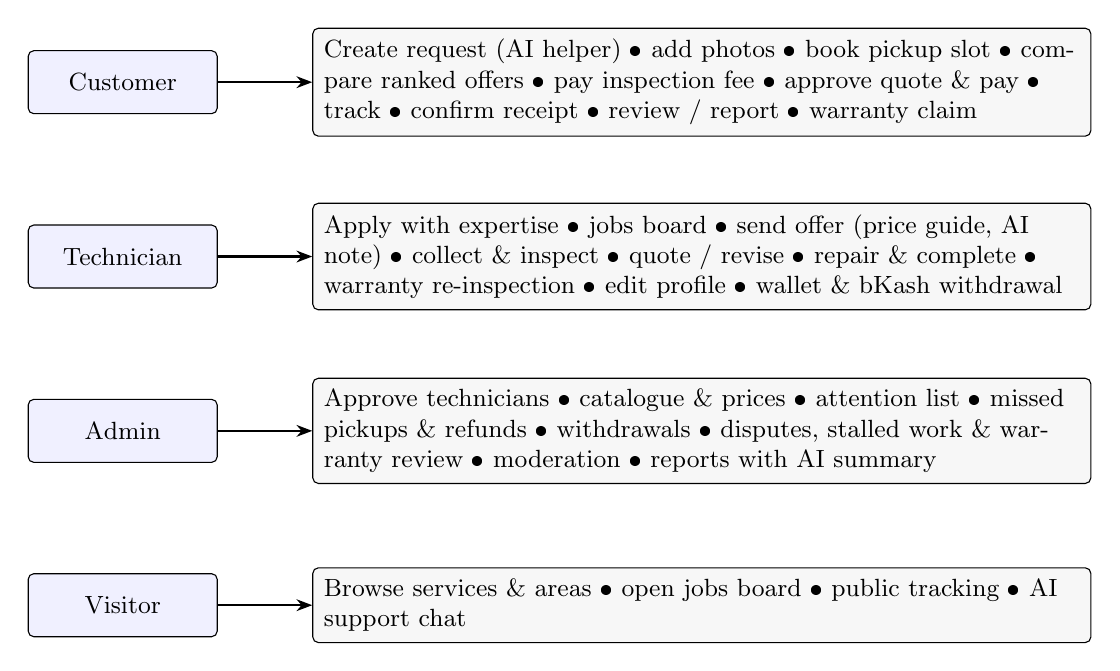
\begin{tikzpicture}[node distance=4mm]
  \node[hl,minimum width=2.4cm] (c) {Customer};
  \node[box,right=12mm of c,text width=9.6cm,align=left] (ca) {Create request (AI helper) \textbullet{} add photos \textbullet{} book pickup slot \textbullet{} compare ranked offers \textbullet{} pay inspection fee \textbullet{} approve quote \& pay \textbullet{} track \textbullet{} confirm receipt \textbullet{} review / report \textbullet{} warranty claim};
  \node[hl,minimum width=2.4cm,below=14mm of c] (t) {Technician};
  \node[box,right=12mm of t,text width=9.6cm,align=left] (ta) {Apply with expertise \textbullet{} jobs board \textbullet{} send offer (price guide, AI note) \textbullet{} collect \& inspect \textbullet{} quote / revise \textbullet{} repair \& complete \textbullet{} warranty re-inspection \textbullet{} edit profile \textbullet{} wallet \& bKash withdrawal};
  \node[hl,minimum width=2.4cm,below=14mm of t] (a) {Admin};
  \node[box,right=12mm of a,text width=9.6cm,align=left] (aa) {Approve technicians \textbullet{} catalogue \& prices \textbullet{} attention list \textbullet{} missed pickups \& refunds \textbullet{} withdrawals \textbullet{} disputes, stalled work \& warranty review \textbullet{} moderation \textbullet{} reports with AI summary};
  \node[hl,minimum width=2.4cm,below=14mm of a] (v) {Visitor};
  \node[box,right=12mm of v,text width=9.6cm,align=left] (va) {Browse services \& areas \textbullet{} open jobs board \textbullet{} public tracking \textbullet{} AI support chat};
  \foreach \x/\y in {c/ca,t/ta,a/aa,v/va} \draw[arr] (\x) -- (\y);
\end{tikzpicture}
\caption{Role-oriented use-case view}
\label{fig:usecase}
\end{figure}

\end{document}
      % Chapter 3 Requirements Analysis
\documentclass{standalone}
\usepackage{standalone}

\begin{document}
\chapter{System Design and Architecture}

\section{High-Level Architecture}
Sarabo has two parts: a client that runs in the browser and an API server. They rely on outside services for identity, payment, storage, email and AI (Figure~\ref{fig:arch}). Both parts run on Vercel. The API is a serverless function in the Mumbai region, close to the MongoDB Atlas cluster that holds all the data, and Vercel also triggers a job once a day.

\begin{figure}[htbp]
\centering
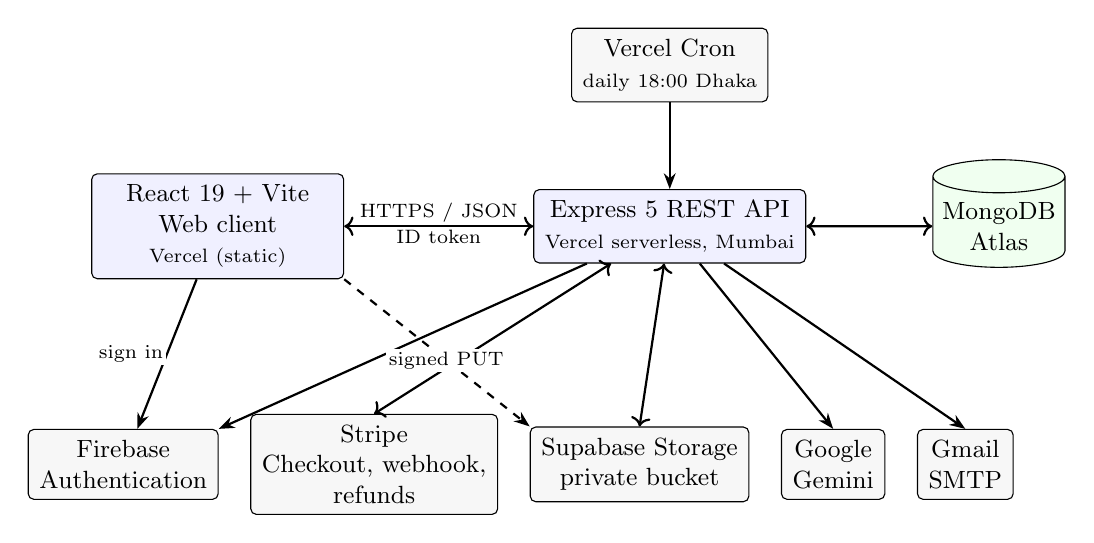
\begin{tikzpicture}[font=\small]
  \node[hl,minimum width=3.2cm] (client) {React 19 + Vite\\Web client\\{\scriptsize Vercel (static)}};
  \node[hl,minimum width=3.2cm,right=2.4cm of client] (api) {Express 5 REST API\\{\scriptsize Vercel serverless, Mumbai}};
  \node[db,right=1.6cm of api] (db) {MongoDB\\Atlas};
  \node[box,below=1.9cm of client,xshift=-1.2cm] (fb) {Firebase\\Authentication};
  \node[box,right=4mm of fb] (stripe) {Stripe\\Checkout, webhook,\\refunds};
  \node[box,right=4mm of stripe] (supa) {Supabase Storage\\private bucket};
  \node[box,right=4mm of supa] (gem) {Google\\Gemini};
  \node[box,right=4mm of gem] (mail) {Gmail\\SMTP};
  \node[box,above=1.1cm of api] (cron) {Vercel Cron\\{\scriptsize daily 18:00 Dhaka}};
  \draw[arr,<->] (client) -- node[lbl,above]{HTTPS / JSON} node[lbl,below]{ID token} (api);
  \draw[arr,<->] (api) -- (db);
  \draw[arr] (client) -- node[lbl,left]{sign in} (fb);
  \draw[arr] (api) -- (fb.north east);
  \draw[arr,<->] (api) -- (stripe.north);
  \draw[arr,<->] (api) -- (supa.north);
  \draw[arr] (api) -- (gem.north);
  \draw[arr] (api) -- (mail.north);
  \draw[arr] (cron) -- (api);
  \draw[arr,dashed] (client.south east) -- node[lbl,pos=0.55]{signed PUT} (supa.north west);
\end{tikzpicture}
\caption{Sarabo high-level architecture}
\label{fig:arch}
\end{figure}

\section{Client Architecture}
The client has about 337 source files, organised into five areas:
\begin{enumerate}
  \item \textbf{Routing and guards}: the public pages (home, services, areas, jobs, tracking, about, become a technician), the sign-in pages, and a dashboard that \texttt{CustomerRoute}, \texttt{TechnicianRoute} and \texttt{AdminRoute} divide by role. The server checks every rule again on its side.
  \item \textbf{Feature components}: the request form and AI helper, photos, pickup slots, offers, inspection, quote, payment, repair, warranty, feedback, wallet, notifications, support chat and administration.
  \item \textbf{Server-state hooks}: TanStack Query with query keys kept in one place, which handles caching, loading and error states, mutations and refreshing only the data that changed.
  \item \textbf{Presentation utilities}: the ``service spine'' that maps each status to a stage, currency formatting, eligibility helpers and an error message for each action.
  \item \textbf{Design system}: shared design tokens, light and dark themes, and Radix UI primitives.
\end{enumerate}

\section{Server Architecture}
The server has about 191 JavaScript files, tests included. It is built in layers: \emph{routes} $\rightarrow$ \emph{middleware} $\rightarrow$ \emph{controllers} $\rightarrow$ \emph{services} / \emph{utilities} $\rightarrow$ \emph{database}. The middleware gives each request an ID, logs it safely, verifies the Firebase token and waits until the database is ready. Each controller is responsible for the state rules of one domain. Services hold the logic that several controllers share, such as eligibility, booking, refunds, settlement, notifications, matching, AI and email. External providers are wrapped in adapters, so the tests can swap them for fakes.

The Stripe webhook route is registered before the JSON parser, because checking the signature needs the raw request body. If the database goes down for a moment, the routes stay registered, so requests fail with a clear 503 error instead of a misleading 404.

\section{Data Collections}
The data is stored in 21 MongoDB collections, listed in Table~\ref{tab:collections}.

\begin{table}[htbp]
\centering
\caption{MongoDB collections}
\label{tab:collections}
\small
\begin{tabularx}{\textwidth}{@{}p{4.6cm}X@{}}
\toprule
\textbf{Collection} & \textbf{Purpose} \\
\midrule
\texttt{users} & Accounts and the authoritative role. \\
\texttt{technicians} & Application, approval status, expertise, region/district, work status, bKash details. \\
\texttt{repair\_requests} & The repair case with all lifecycle sub-documents. \\
\texttt{job\_applications} & Technician offers on open requests and their states. \\
\texttt{service\_definitions} & Versioned catalogue of services and prices. \\
\texttt{payments} & Stripe payment rows for inspection fees and repairs, including refund state. \\
\texttt{checkout\_sessions} & Checkout idempotency and expiry. \\
\texttt{technician\_withdrawals} & Withdrawal requests and admin processing. \\
\texttt{technician\_reviews} & Customer ratings with moderation history. \\
\texttt{technician\_reports} & Private customer reports with status and admin notes. \\
\texttt{notifications} & In-app notifications with de-duplication keys. \\
\texttt{tracking\_events} & Sanitized public timeline. \\
\texttt{damage\_upload\_sessions} & Customer photo upload sessions. \\
\texttt{repair\_evidence\_sessions} & Technician completion-evidence sessions. \\
\texttt{deletion\_cleanups} & Retry records for storage clean-up after deletion. \\
\texttt{turned\_away\_requests} & Hashed count of refused demand (180-day expiry). \\
\texttt{email\_log} & Sent/failed email record (90-day expiry). \\
\texttt{support\_rate\_limits} & Shared AI rate-limit counters (auto-expiring). \\
\texttt{ai\_report\_summaries} & Last AI summary per report period. \\
\texttt{warranty\_claims} & Warranty claims with their full decision and refund history. \\
\texttt{warranty\_photo\_uploads} & Short-lived upload sessions for warranty photos. \\
\bottomrule
\end{tabularx}
\end{table}

\section{Repair Request Document}
Each request has \texttt{schemaVersion: 2}, a \texttt{product} snapshot (category, brand and model) and its own copy of the chosen service with its price rule. Because of this copy, editing the catalogue later never changes a request that already exists (Figure~\ref{fig:requestdoc}).

\begin{figure}[htbp]
\centering
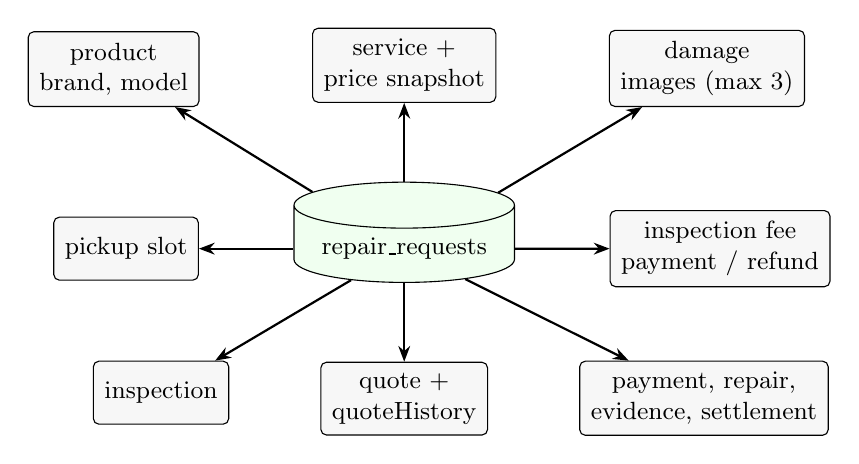
\begin{tikzpicture}[font=\small]
  \node[db,minimum width=2.8cm] (r) {repair\_requests};
  \node[box,above left=10mm and 18mm of r] (p) {product\\brand, model};
  \node[box,above=10mm of r] (s) {service +\\price snapshot};
  \node[box,above right=10mm and 18mm of r] (d) {damage\\images (max 3)};
  \node[box,left=12mm of r] (pk) {pickup slot};
  \node[box,right=12mm of r] (ip) {inspection fee\\payment / refund};
  \node[box,below left=10mm and 18mm of r] (i) {inspection};
  \node[box,below=10mm of r] (q) {quote +\\quoteHistory};
  \node[box,below right=10mm and 18mm of r] (rp) {payment, repair,\\evidence, settlement};
  \foreach \n in {p,s,d,pk,ip,i,q,rp} \draw[arr] (r) -- (\n);
\end{tikzpicture}
\caption{Conceptual structure of a V2 repair request}
\label{fig:requestdoc}
\end{figure}

\section{State Model}
The status field, \texttt{deliveryStatus}, and several of its values come from the parcel-delivery codebase that Sarabo started from. I kept them as a fixed internal contract, and users only ever see repair terms (Table~\ref{tab:states}).

\begin{table}[htbp]
\centering
\caption{Repair lifecycle states}
\label{tab:states}
\small
\begin{tabularx}{\textwidth}{@{}p{4.4cm}X@{}}
\toprule
\textbf{Stored state} & \textbf{Meaning shown to users} \\
\midrule
\texttt{pending-pickup} & Waiting for a technician; open on the jobs board. \\
\texttt{assignment\_pending} & Offered directly by an admin; technician to accept or reject. \\
\texttt{driver\_assigned} & Technician booked. \\
\texttt{rider\_arriving} & Technician on the way. \\
\texttt{parcel\_picked\_up} & Device collected. \\
\texttt{inspection\_completed} & Inspection submitted. \\
\texttt{quote\_submitted} & Final price waiting for the customer. \\
\texttt{quote\_approved} & Customer accepted the price. \\
\texttt{quote\_rejected} & Customer declined the price. \\
\texttt{payment\_completed} & Customer paid. \\
\texttt{repair\_in\_progress} & Repair underway. \\
\texttt{repair\_completed} & Repair finished; waiting for hand-over. \\
\texttt{parcel\_delivered} & Customer confirmed receipt (terminal). \\
\texttt{cancelled} & Ended through an allowed path. \\
\bottomrule
\end{tabularx}
\end{table}

Other records have their own, smaller sets of states. A job application (an offer) can be \texttt{pending}, \texttt{accepted}, \texttt{not\_chosen}, \texttt{withdrawn}, \texttt{no\_show} or \texttt{declined}. A settlement goes from \emph{pending} to \emph{available}, or to \emph{reversed} after a refund. A warranty claim starts as \emph{submitted}, goes through re-inspection and a decision, and ends as \emph{resolved} or \emph{refunded}. A withdrawal goes from \emph{requested} to either \emph{paid} or \emph{rejected}.

\section{The Service Spine}
That many states would be hard for a customer to follow, so the interface groups them into four stages that are easy to understand (Figure~\ref{fig:spine}). These stages appear on the home page, the tracking page and every dashboard. Confirming receipt is not a fifth stage. It is the hand-over action that comes after ``Repaired''.

\begin{figure}[htbp]
\centering
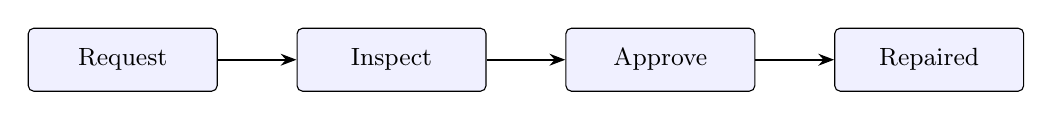
\begin{tikzpicture}[node distance=10mm]
  \node[hl,minimum width=2.4cm] (a) {Request};
  \node[hl,minimum width=2.4cm,right=of a] (b) {Inspect};
  \node[hl,minimum width=2.4cm,right=of b] (c) {Approve};
  \node[hl,minimum width=2.4cm,right=of c] (d) {Repaired};
  \draw[arr] (a)--(b); \draw[arr] (b)--(c); \draw[arr] (c)--(d);
\end{tikzpicture}
\caption{The four-stage service spine shown to users}
\label{fig:spine}
\end{figure}

\section{API Design}
The API has more than 120 endpoints, grouped into families by resource. Table~\ref{tab:api} shows some typical ones, and Appendix~\ref{app:api} gives a longer list.

\begin{table}[htbp]
\centering
\caption{Representative API endpoints}
\label{tab:api}
\footnotesize
\begin{tabularx}{\textwidth}{@{}p{1.2cm}p{8cm}X@{}}
\toprule
\textbf{Method} & \textbf{Route} & \textbf{Purpose} \\
\midrule
POST & \nolinkurl{/repair-requests} & Create a request \\
GET & \nolinkurl{/jobs} & Public open-jobs board \\
POST & \nolinkurl{/repair-requests/:id/applications} & Technician sends an offer \\
POST & \nolinkurl{/repair-requests/:id/applications/:aid/accept} & Customer chooses an offer \\
POST & \nolinkurl{/repair-requests/:id/inspection} & Submit inspection \\
POST & \nolinkurl{/repair-requests/:id/quote/decision} & Approve or reject quote \\
POST & \nolinkurl{/repair-requests/:id/checkout-session} & Start repair payment \\
POST & \nolinkurl{/stripe-webhook} & Signed payment events \\
POST & \nolinkurl{/repair-requests/:id/repair/complete} & Complete repair \\
POST & \nolinkurl{/repair-requests/:id/review} & Rate the technician \\
POST & \nolinkurl{/ai/request-draft} & AI request helper \\
GET & \nolinkurl{/admin/attention} & Items needing admin action \\
GET & \nolinkurl{/public/trackings/:code} & Sanitized tracking \\
\bottomrule
\end{tabularx}
\end{table}

\end{document}
      % Chapter 4 System Design and Architecture
\documentclass{standalone}
\usepackage{standalone}

\begin{document}
\chapter{Implementation}

\section{Technology Stack}
\begin{table}[htbp]
\centering
\caption{Implemented technology stack}
\label{tab:stack}
\small
\begin{tabularx}{\textwidth}{@{}p{2.6cm}p{4.4cm}X@{}}
\toprule
\textbf{Layer} & \textbf{Technology} & \textbf{Role in Sarabo} \\
\midrule
Frontend & React 19, Vite 7 & Component-based single-page app and build tooling \\
Routing & React Router 7 & Public, authenticated and role-specific routes \\
Server state & TanStack Query 5, TanStack Table & Caching, mutations, invalidation; admin data tables \\
UI & Tailwind CSS 4, Radix UI, Motion, Recharts, Leaflet & Design system, accessible primitives, animation, charts, service-area map \\
Forms & react-hook-form & Validated multi-step forms \\
Backend & Node.js, Express 5 & REST API, middleware, controllers, services \\
Database & MongoDB 7 driver, MongoDB Atlas & Persistence and multi-document transactions \\
Identity & Firebase Authentication + Admin SDK & Sign-in (email, Google) and token verification \\
Payments & Stripe 20 & Checkout, signed webhooks, refunds \\
Storage & Supabase Storage & Private images with signed URLs \\
AI & Google Gemini (\texttt{@google/genai}) & Support chat, request helper, offer note, report summary \\
Email & Nodemailer (Gmail) & Request, reminder and job-offer emails \\
Documents & pdfkit & PDF payment receipts \\
Testing & Custom Node test harness, Playwright & Server integration tests; browser tests \\
Delivery & GitHub Actions, Vercel & CI, serverless API (Mumbai region), cron, static hosting \\
\bottomrule
\end{tabularx}
\end{table}

\section{Development Process}
I built Sarabo in small phases that were each easy to review, from 26 July to 4 October 2026, followed by a final improvement phase from 11 to 16 October. Altogether this came to 163 commits on the client and 120 on the server. Every phase followed the same loop. First I defined the rule, then implemented it on the server together with its tests, then built the interface, ran lint, the build and the tests, and finally reviewed the result. Larger features were developed on their own branches and merged through a pull request once CI had passed (Table~\ref{tab:phases}).

\begin{longtable}{@{}p{3.2cm}p{2.2cm}p{8.8cm}@{}}
\caption{Development phases (from the git history)}\label{tab:phases}\\
\toprule
\textbf{Phase} & \textbf{Dates} & \textbf{Main work} \\
\midrule
\endfirsthead
\toprule
\textbf{Phase} & \textbf{Dates} & \textbf{Main work} \\
\midrule
\endhead
\bottomrule
\endfoot
1. Foundation and hardening & 26--28 Jul & Imported the base codebase; secured authentication and role routing; secure Stripe checkout and webhook; validated status transitions; public sanitized tracking; transactional assignment, approval and completion. \\
2. Admin and notifications & 29 Jul -- 4 Aug & Admin request management; in-app notifications; production database isolation; health monitoring; double-booking prevention. \\
3. Repair domain (V2) & 5--8 Aug & Service taxonomy and priced catalogue; technician expertise; V2 request schema; expertise-based matching; damage uploads; prices in BDT; inspection, quote, payment and repair workflows; safe deletion; verified email. \\
4. Rename to Sarabo & 10--12 Aug & Migrated database, collections, fields, modules, API routes and UI from parcel to repair vocabulary; assignment accept/reject; receipt confirmation. \\
5. Money and UI redesign & 13--19 Aug & 90/10 settlement; wallet and withdrawals; storage moved to Supabase; complete ``service spine'' redesign; accessibility pass. \textit{(Earlier report submitted 20 Aug.)} \\
6. AI support and feedback & 18--24 Sep & Gemini support chat; reviews and private reports with moderation; product tour; second redesign; admin catalogue editor; CI on GitHub Actions. \\
7. Operations & 24--25 Sep & Pickup scheduling; region rule; email updates; Playwright tests; admin reports and attention list; in-app reminders; refusing unmatchable requests. \\
8. Job portal and inspection fee & 25 Sep -- 2 Oct & Technician offers and customer choice; inspection-fee payment, credit, refunds and split; reject-and-repost; public jobs board; job notifications; PDF receipts; one-step approve-and-pay. \\
9. AI helpers and payouts & 2--4 Oct & AI request helper (text and photo); price guide and AI offer note; AI report summary; bKash withdrawals; hosting configuration. \\
10. Final improvements & 11--16 Oct & Map search, final payout on removal, faster API and AI, offer ranking, warranty, deadlines for every waiting state, pickup condition, minimum inspection fee, technician profile editing (Section~\ref{sec:finalphase}). \\
\end{longtable}

\section{Frontend Implementation}
\subsection{Role-Aware Routing}
The dashboard is behind a route that requires sign-in, with guards for each role. Customers see Overview, Create Request, My Requests and Payment History. Technicians see Overview, Find jobs, Assigned jobs, Completed jobs, Warranty claims and Wallet. Admins see Overview, Repair requests, Assign technicians, Technicians, Withdrawals, Warranty claims, Users, Services \& prices, Reports, Technician reports and Technician reviews. Every role also has Notifications and Profile, and on phones these pages move to a tab bar at the bottom. Deep links such as \texttt{?category=smartphone} are kept through sign-in. The routing is only there for convenience, though. Every protected endpoint checks authentication and authorization again on the server.

\subsection{Server-State Hooks}
Each feature has its own query-key factory (for example \texttt{quoteKeys} or \texttt{walletKeys}) and hooks for reading and changing data. When something changes, only the queries that are now out of date are refreshed. Approving a quote, for instance, refreshes the quote, the request, the request list and the payment eligibility. This keeps what all three roles see in step, without anyone having to reload the page.

\subsection{Action-First Workspace}
Every request page (see Figure~\ref{fig:wt-c10} for an example) starts with the service spine. Below it is a ``next step'' panel that tells the signed-in user what to do, such as ``Choose a technician'' or ``Approve and pay BDT 3,800'', and the supporting details come after that. Shared components for empty, loading, error and confirmation states and for forms make every page behave the same way. A product tour introduces each dashboard, and a command menu lets users move around with the keyboard.

\section{Backend Implementation}
\subsection{Controllers, Services and Adapters}
Each domain has a controller for its endpoints, for example \texttt{jobPortalController}, \texttt{quoteController} and \texttt{paymentController}. Logic that is shared goes into services such as \texttt{jobBooking}, \texttt{inspectionFeeRefunds}, \texttt{paymentEligibility}, \texttt{technicianMatchGate} and \texttt{notificationService}. The external providers (Supabase, Gemini and Stripe) are wrapped in adapters, which the tests replace with fakes.

\subsection{Database Transactions}
Whenever several records depend on each other, they are updated inside a MongoDB transaction. Take booking after an inspection-fee payment. In one transaction (\texttt{services/\allowbreak jobBooking.js}) the server records the payment, sets the request to \texttt{driver\_assigned}, marks the technician as busy, accepts the chosen offer and marks all the other offers \texttt{not\_chosen}. If any of these steps fails, none of them is saved.

\subsection{Notifications, Email and Scheduled Jobs}
All in-app notifications are created through one service. Each one has a de-duplication key, so retrying an action never sends the same notification twice. Emails (request received, pickup reminder and new job) are sent through Gmail after the main action has finished. If an email fails, it is logged in \texttt{email\_log}, and the request itself still succeeds.

Once a day a Vercel Cron job calls \texttt{GET /cron/pickup-reminders} at 12:00 UTC, which is 18:00 in Bangladesh. The call is protected by a secret. The job sends the pickup reminders for the next day and applies every deadline described in Section~\ref{sec:nostuck}. It closes declined and unpaid quotes that nobody acted on, confirms receipts that the customer has left unanswered for three days, and warns admins about late warranty steps and stalled work. Each of these steps runs separately, so if one fails the others still run. Email and the daily job are both turned on in production, which means the live site sends reminders by email as well as in the app.

\section{Service Catalogue and Matching}
Admins edit services and prices from the dashboard. Changing a price increases \texttt{pricingRule.version}, while requests that already exist keep their own copy of the old price. Every service has an inspection fee of at least 100\,BDT, or 200\,BDT if the top of its estimate is above 1,000\,BDT. A single rule, \texttt{minimumInspectionFee}, is used for requests, offers, the catalogue editor and the public price list. A one-time migration raised the fee for the 16 live services that had none.

When a request is created, \texttt{technicianMatchGate} checks that there is an approved technician in the region who covers the device and the repair at the required level. If there is not, the API answers \texttt{409 NO\_TECHNICIAN\_AVAILABLE}, and the refused request is counted once per customer, service, region and day, with the customer stored only as a hash. These counts show admins where they need to recruit more technicians.

\section{Pickup Scheduling}
Customers choose one of four two-hour windows between 10:00 and 18:00 Bangladesh time, from Saturday to Thursday, anywhere from one hour to seven days ahead. Each region accepts a set number of pickups per slot. This number can be configured and is three by default, and a full slot returns \texttt{409 PICKUP\_SLOT\_FULL}. The customer can change the window until the device is collected, and if the pickup moves, the reminder is sent again.

\section{Quotation Model}
A quote is made up of labour, parts and additional charges, all in whole taka, plus a total, a currency, a version and a status. When a quote is rejected, it is moved to \texttt{quoteHistory} before the live quote is cleared. That way there is still a record of it, and it can never be paid by mistake.

\begin{lstlisting}[caption={Quote total and amount still to pay},label={lst:quote}]
repairSubtotal   = laborAmount + partsAmount + additionalCharges
quote.totalAmount = repairSubtotal            (currency "BDT")
amountDue        = max(quote.totalAmount - inspectionFeePaid, 0)
\end{lstlisting}

\section{Payment Implementation}
Every Stripe Checkout session is created from data the server has stored, either the approved quote or the fee of the chosen offer. It never uses an amount sent by the browser. The session's metadata records what it is paying for, either \texttt{repair} or \texttt{inspection\_fee}. The signed webhook and, as a backup, the success page both call the same idempotent processor, so each payment is recorded exactly once. A single server function decides whether a request counts as paid, and the eligibility checks, admin filters and status badges all use it. Every payment also has a PDF receipt showing the Stripe ID, the date in Dhaka time, the device, the repair, the technician, the amount and the refund status.

\section{Technician Settlement and Wallet}
As soon as a repair is paid, the server takes a snapshot of the settlement from the approved quote, and this snapshot does not change afterwards:

\begin{lstlisting}[caption={Settlement rule (whole taka)},label={lst:settlement}]
commission  = round(repairSubtotal * 10 / 100)    # Sarabo
receivable  = repairSubtotal - commission          # Technician
# invariant: commission + receivable == repairSubtotal
\end{lstlisting}

The settlement stays \emph{pending} until the customer confirms they have received the device, and then it becomes \emph{available}. Balances are never stored. They are worked out each time from the settlements and withdrawals, so they cannot slowly drift away from the truth. A technician can withdraw up to their available balance to a bKash number. An admin then sends the money with bKash Send Money and records the TrxID. A unique partial index makes sure each technician can only have one open withdrawal at a time.

\section{Damage and Evidence Images}
Images go straight from the browser to a private Supabase bucket through a signed upload URL. They must be JPEG, PNG or WebP files of up to 8\,MB, with at most three per request. Before attaching an image, the server checks the real type and size of the stored file. Signed links for viewing it last five minutes and are given only to the owner, an admin or the assigned technician. When something is deleted, the storage clean-up is retried until it succeeds.

\section{Public Tracking and Jobs Board}
Every request gets a tracking code of the form \texttt{SRB-<random>}, with 128 bits of randomness. \texttt{GET /public/trackings/:code} only accepts exact codes, is rate limited, and returns nothing but the status timeline. The jobs board (\texttt{GET /jobs}, limited to 60 requests per minute per address) shows the device, the repair, the area, the pickup day, the usual price and the number of offers. It never shows the problem description, photos, the tracking code or any personal details.

\section{Deployment and Continuous Integration}
The API is a Vercel serverless function (Node.js 24) at \url{https://sarabo-server.vercel.app}, and the client is a static Vercel site at \url{https://sarabo-client-six.vercel.app}. Both are deployed from the \texttt{main} branch. The API runs in Vercel's Mumbai region (\texttt{bom1}), close to the MongoDB Atlas cluster. Moving it there brought the first request after an idle period down from 10.7\,s to 2.9\,s, and a normal request from 0.75\,s to about 0.2\,s. Production has a database of its own, and the server refuses to start there unless its secrets and an \texttt{https} client origin are set.

GitHub Actions runs on every push. It runs the server suites on a throwaway MongoDB replica set, never with real credentials, and it runs lint, the build and the browser tests for the client. I only push to \texttt{main} after all of these checks have passed.

\section{Final Improvement Phase}
\label{sec:finalphase}
The features were finished on 4 October. After that, a final phase from 11 to 16 October 2026 got the project ready for submission. It began with a review of both codebases and a fresh run of every check (Chapter~\ref{ch:testing}). I recorded each change in the project work log, with the problem it solved, the files it touched and how it was verified. Table~\ref{tab:finalphase} summarises these changes.

{\small
\begin{longtable}{@{}p{0.6cm}p{2cm}p{11.4cm}@{}}
\caption{Final improvement phase log}\label{tab:finalphase}\\
\toprule
\textbf{\#} & \textbf{Date} & \textbf{Change and verification} \\
\midrule
\endfirsthead
\toprule
\textbf{\#} & \textbf{Date} & \textbf{Change and verification} \\
\midrule
\endhead
\bottomrule
\endfoot
0 & 11 Oct 2026 & Codebase and documentation review; re-ran server suites against an isolated in-memory MongoDB replica set, client lint, production build and Playwright browser tests. \\
1 & 11 Oct 2026 & Service-area map: OpenStreetMap coordinates for 226 of the 236 covered sub-areas, each kept only if it lies inside its own district. Searching a sub-area (e.g.\ Ambarkhana) now zooms to that spot instead of the district centre. Verified with two new browser tests on desktop and mobile. \\
2 & 11 Oct 2026 & Final payout on technician removal: removing a technician queues their whole available balance as a bKash withdrawal in the same transaction (Section~\ref{sec:removalpayout}). Verified with 15 new server checks. \\
3 & 11 Oct 2026 & Homepage hero: the photo moved to the right side (top band on phones) so the headline no longer sits over it. Checked with screenshots at three screen widths. \\
4 & 11 Oct 2026 & Final verification of the committed code and CI on both repositories (Section~\ref{sec:results}). \\
5 & 14 Oct 2026 & Slow first load: the API was moved to Vercel's Mumbai region, next to the database (10.7\,s $\rightarrow$ 2.9\,s cold, 0.75\,s $\rightarrow$ 0.2\,s warm, measured live). \\
6 & 14 Oct 2026 & AI support timeouts: faster Gemini model with an automatic fallback model; live answers now take 1.4--1.9\,s. 4 new tests. \\
7 & 14 Oct 2026 & Smarter matching: offers ranked by rating, reliability, price, district and reply time, with a ``Best match'' badge and reasons (Section~\ref{sec:ranking}). 22 new tests. \\
8 & 14 Oct 2026 & 30-day repair warranty with free re-inspection, re-repair, admin review and refunds (Section~\ref{sec:warranty}). 45 new tests. \\
9 & 14 Oct 2026 & Whole-workflow review, then fixes so no request can get stuck: unpaid quotes, not-repairable devices, repairs that cannot be finished, unconfirmed receipt, warranty deadlines (Section~\ref{sec:nostuck}). 42 new tests. \\
10 & 14 Oct 2026 & Remaining gaps: late payment after cancellation refunded, device return after cancellation, stalled-work alerts, pickup condition, customer not home. 30 new tests. \\
11 & 14 Oct 2026 & Photos upload only when the customer presses ``Upload''; technicians edit their own profile; minimum inspection fee for every repair, applied to old offers and migrated on production. 22 new tests. \\
12 & 14 Oct 2026 & All of the above pushed and deployed; full verification (Section~\ref{sec:results}) and screenshots of the running system (Chapter~\ref{ch:walkthrough}). \\
13 & 16 Oct 2026 & Stripe's repair-payment page named the item ``Repair request: undefined''; it now names the device (``Repair: Samsung Galaxy A54''). 1 new test; pushed and deployed. \\
\end{longtable}
}

\end{document}
      % Chapter 5 Implementation
\documentclass{standalone}
\usepackage{standalone}

\begin{document}
\chapter{Core Workflows and Business Rules}

\section{End-to-End Repair Workflow}
Figure~\ref{fig:e2e} shows the main path of a repair, from request to settlement.

\begin{figure}[htbp]
\centering
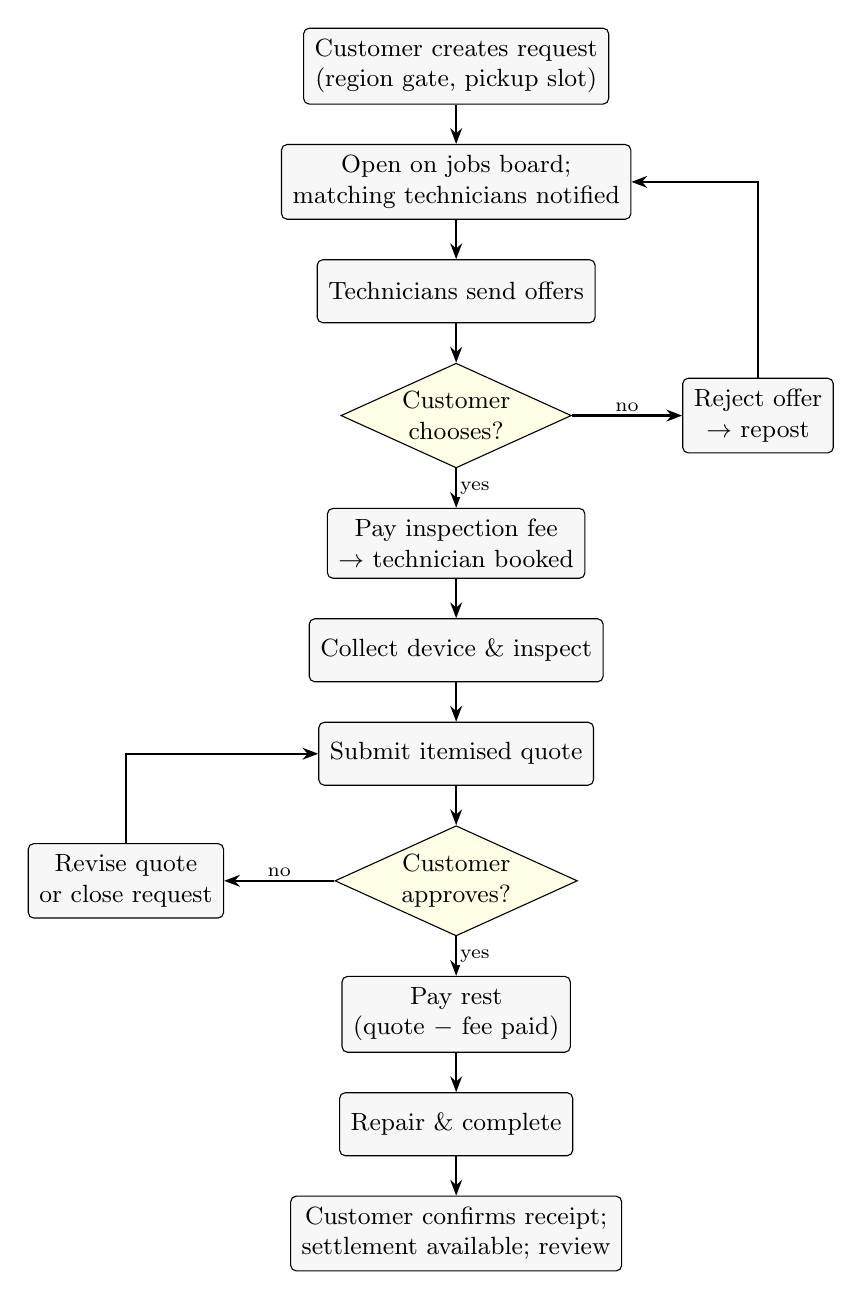
\begin{tikzpicture}[node distance=5mm and 8mm,font=\small]
  \node[box] (a) {Customer creates request\\(region gate, pickup slot)};
  \node[box,below=of a] (b) {Open on jobs board;\\matching technicians notified};
  \node[box,below=of b] (c) {Technicians send offers};
  \node[dec,below=of c] (d) {Customer\\chooses?};
  \node[box,right=14mm of d] (rj) {Reject offer\\$\rightarrow$ repost};
  \node[box,below=of d] (e) {Pay inspection fee\\$\rightarrow$ technician booked};
  \node[box,below=of e] (f) {Collect device \& inspect};
  \node[box,below=of f] (g) {Submit itemised quote};
  \node[dec,below=of g] (h) {Customer\\approves?};
  \node[box,left=14mm of h] (rv) {Revise quote\\or close request};
  \node[box,below=of h] (i) {Pay rest\\(quote $-$ fee paid)};
  \node[box,below=of i] (j) {Repair \& complete};
  \node[box,below=of j] (k) {Customer confirms receipt;\\settlement available; review};
  \draw[arr] (a)--(b); \draw[arr] (b)--(c); \draw[arr] (c)--(d);
  \draw[arr] (d)--node[lbl,right]{yes}(e); \draw[arr] (d)--node[lbl,above]{no}(rj);
  \draw[arr] (rj) |- (b);
  \draw[arr] (e)--(f); \draw[arr] (f)--(g); \draw[arr] (g)--(h);
  \draw[arr] (h)--node[lbl,above]{no}(rv); \draw[arr] (rv) |- (g);
  \draw[arr] (h)--node[lbl,right]{yes}(i); \draw[arr] (i)--(j); \draw[arr] (j)--(k);
\end{tikzpicture}
\caption{End-to-end repair workflow}
\label{fig:e2e}
\end{figure}

\section{Request Creation}
The customer chooses a device category and a repair service from the live catalogue (or lets the AI helper propose them), adds brand, model and a description, optionally adds up to three photos (shown as previews and sent only when the customer presses ``Upload''), and picks a pickup window. The estimate card shows the catalogue's price range. Before submitting, the form calls \texttt{GET /service-availability}; the server repeats the check on submission and refuses the request with a clear explanation if no approved technician in that region can do this repair at the required level. Accepted requests receive a tracking code and a confirmation email (Figures~\ref{fig:scr-c02-ai-helper}--\ref{fig:scr-c04-created}).

\section{Job Portal and Offers}
A request is \emph{open} while it is waiting for a technician. It appears on the public jobs board as a safe summary, and every approved technician who matches it receives a \texttt{job\_posted} notification (at most once per request). A technician who starts matching later, after being approved or adding a skill, is told about the open jobs they can now take. Approved technicians see the details they need (district, pickup time, problem description and photos) but never the customer's name, email or street address.

A technician sends an \emph{offer}: an estimate range, an inspection fee (at least the minimum fee and at most the catalogue fee for that service) and a note. The customer compares offers side by side and either chooses one or rejects one with a reason (price, inspection fee or other). A rejected offer causes the job to be \emph{reposted} to the top of the board; the rejected technician may send one revised offer, and other matching technicians are notified. If no offer is waiting 24 hours after the job was last posted, it appears on the admin attention list. Admins can also invite a specific technician to apply, or assign one directly as an override. Figures~\ref{fig:scr-t03-offer} and~\ref{fig:scr-c06-offers} show an offer being sent and compared.

\section{Offer Ranking (Smarter Matching)}
\label{sec:ranking}
When several technicians send offers, the customer sees them ranked rather than in arrival order. A pure scoring module (\texttt{services/offerRanking.js}) combines five factors, all from data Sarabo already stores, so no paid service, map API or AI is needed (Table~\ref{tab:ranking}). A technician with no history gets a neutral score for that factor, neither a penalty nor a bonus. The top offer gets a ``Best match'' badge (only when there are at least two), and short reasons are shown only when they are true, for example ``Rated 4.8\,$\star$ from 12 reviews'' or ``In your district''. The customer can also sort by lowest price or newest, and always makes the final choice; nothing is booked automatically.

\begin{table}[htbp]
\centering
\caption{Offer ranking factors}
\label{tab:ranking}
\small
\begin{tabularx}{\textwidth}{@{}p{2.6cm}cX@{}}
\toprule
\textbf{Factor} & \textbf{Weight} & \textbf{How it is measured} \\
\midrule
Rating & 30\% & Average review, smoothed toward 3\,$\star$ so one 5\,$\star$ review does not beat forty 4.8\,$\star$ reviews \\
Reliability & 25\% & Repairs completed compared with missed pickups \\
Price & 20\% & The offer's estimate compared with the other offers on the same job \\
District & 15\% & Same district as the customer \\
Reply time & 10\% & Median minutes from the job being posted to the technician's offer (last 20 offers, at least 3) \\
\bottomrule
\end{tabularx}
\end{table}

\section{Inspection Fee and Booking}
Choosing an offer with a fee opens a Stripe Checkout for exactly that fee; nothing is booked yet. When Stripe confirms the payment, one transaction records it and books the technician. If the technician can no longer be booked at that moment (busy, request cancelled, someone else chosen), the payment is recorded and refunded automatically and the customer is asked to choose again. The fee is stored separately from the repair payment and is later credited toward the final price (Figures~\ref{fig:scr-c07-choose}--\ref{fig:scr-c09-booked} and~\ref{fig:scr-c10-quote}). Table~\ref{tab:feeoutcomes} shows what happens to the fee when the repair does not go ahead.

\begin{table}[htbp]
\centering
\caption{Inspection fee outcomes}
\label{tab:feeoutcomes}
\small
\begin{tabularx}{\textwidth}{@{}Xp{5.8cm}@{}}
\toprule
\textbf{Situation} & \textbf{Fee} \\
\midrule
Repair approved and paid & Credited toward the final price \\
Technician does not come (admin records a missed pickup) & Full refund; other offers can be chosen \\
Customer cancels 2 hours or more before the pickup window & Full refund \\
Customer cancels less than 2 hours before & Kept: 90\% technician, 10\% Sarabo \\
Customer declines the final price and the request ends & Kept: 90\% technician, 10\% Sarabo \\
Booking fails after payment & Automatic full refund \\
\bottomrule
\end{tabularx}
\end{table}

Refunds happen in two steps. Inside the transaction that causes the refund, the fee and its payment row are marked \emph{refund pending}. After the transaction commits, Stripe is asked to refund with the idempotency key \texttt{inspection-refund-<session id>}, which guarantees at most one refund. If Stripe fails, the refund stays pending, appears on the admin home page, and can be retried with one click; it is never silently lost.

\section{Inspection, Quotation and Revision}
After collecting the device, only the booked technician can submit the inspection, which records findings and detected issues. The quote can be submitted only from \texttt{inspection\_completed}. The customer sees the quote together with the fee already paid and the amount still due, and the approve button reads ``Approve and pay BDT \textit{X}'', so approval leads straight to payment.

If the customer rejects the quote, the technician may revise or close the request (Figure~\ref{fig:revise}). Revising archives the old quote and reuses the normal submit-and-decide cycle. If the technician neither revises nor closes within three days, the daily job closes the request automatically; the request records who closed it (\texttt{technician}, \texttt{customer} or \texttt{auto}), and the inspection fee is kept and split.

\begin{figure}[htbp]
\centering
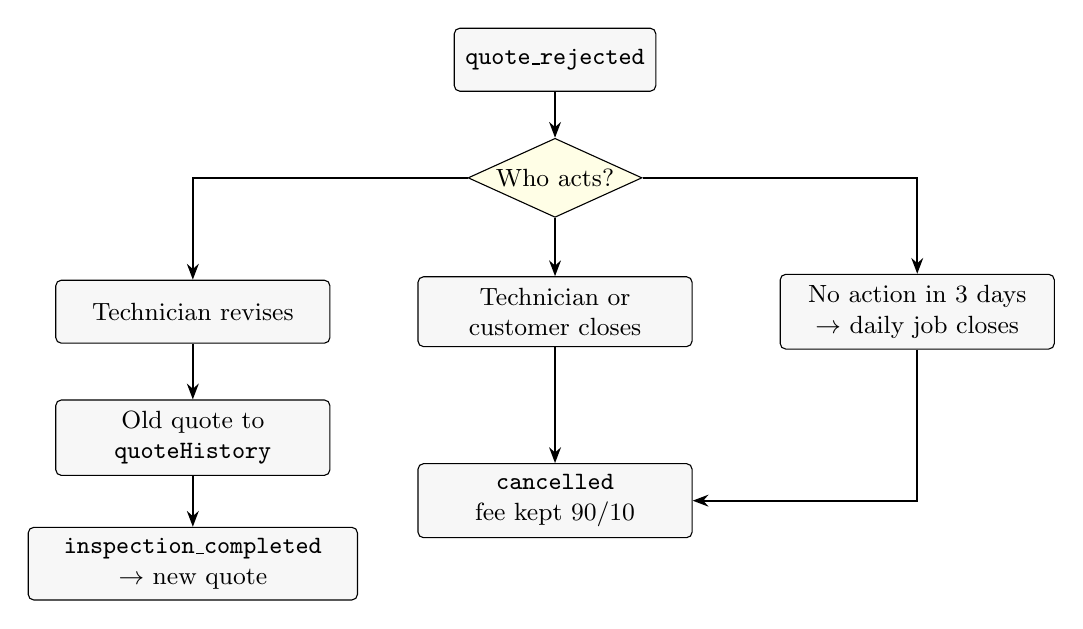
\begin{tikzpicture}[font=\small]
  \node[box] (r) at (0,0) {\texttt{quote\_rejected}};
  \node[dec] (d) at (0,-1.5) {Who acts?};
  \node[box,text width=3.2cm] (rv) at (-4.6,-3.2) {Technician revises};
  \node[box,text width=3.2cm] (tc) at (0,-3.2) {Technician or\\customer closes};
  \node[box,text width=3.2cm] (au) at (4.6,-3.2) {No action in 3 days\\$\rightarrow$ daily job closes};
  \node[box,text width=3.2cm] (ar) at (-4.6,-4.8) {Old quote to\\\texttt{quoteHistory}};
  \node[box,text width=3.9cm] (ic) at (-4.6,-6.4) {\texttt{inspection\_completed}\\$\rightarrow$ new quote};
  \node[box,text width=3.2cm] (cl) at (0,-5.6) {\texttt{cancelled}\\fee kept 90/10};
  \draw[arr] (r)--(d); \draw[arr] (d)-|(rv); \draw[arr] (d)--(tc); \draw[arr] (d)-|(au);
  \draw[arr] (rv)--(ar); \draw[arr] (ar)--(ic); \draw[arr] (tc)--(cl); \draw[arr] (au)|-(cl);
\end{tikzpicture}
\caption{Rejected-quote recovery}
\label{fig:revise}
\end{figure}

Each quote round has its own notification identity, derived on the server as \texttt{quoteHistory.length + 1}. A retried submission of the same round is therefore harmless, while a genuine revision produces a new notification (see Appendix~\ref{app:incident}).

\section{Payment, Repair and Receipt}
Payment is possible only for an approved quote that is not yet paid. After payment the technician starts the repair, adds progress updates and completes it, optionally with evidence photos. Completion releases the technician for other work and shows the customer a ``Confirm receipt'' action. Only that confirmation moves the request to its terminal state and makes the technician's earning available, so a technician cannot withdraw money for a device the customer has not received.

\section{No Request Can Get Stuck}
\label{sec:nostuck}
A review of the whole workflow before the final release looked for real-life situations in which a request could wait forever. Each one now has a way out, an automatic step after a deadline, or an admin alert (Table~\ref{tab:nostuck}). A daily scheduled job applies the deadlines, and a single rule set (\texttt{services/stalledWork.js}) shows any work that has not moved on in three days (fourteen for a running repair) on the admin overview.

\begin{longtable}{@{}p{4.4cm}p{9.8cm}@{}}
\caption{Situations that used to block a request, and how they end now}\label{tab:nostuck}\\
\toprule
\textbf{Situation} & \textbf{What happens now} \\
\midrule
\endfirsthead
\toprule
\textbf{Situation} & \textbf{What happens now} \\
\midrule
\endhead
\bottomrule
\endfoot
Approved quote never paid & Customer can cancel (``I don't want the repair''); otherwise closed automatically after 3 days. The inspection fee is kept 90/10 and the technician is freed. \\
Device not repairable or not worth it & Technician or customer closes the request; same fee outcome. \\
Paid repair cannot be finished & Technician reports why; an admin cancels and refunds the whole amount, and the technician's settlement is reversed. \\
Customer never confirms receipt & Technician marks the device returned; receipt is confirmed automatically after 3 days unless the customer says ``I haven't received it'', which goes to an admin. \\
Device must go back after a cancellation & The return is recorded, confirmed by the customer or automatically after 3 days; disputes go to an admin. \\
Customer not at home at pickup & Technician reports it; the customer is asked for a new time. It is not counted as a technician no-show. \\
Payment arrives after cancellation & Recorded and refunded at once; a failed refund stays on the admin refund list. \\
Work not moving (no inspection, quote, answer or repair) & Shown on the admin overview with one alert per request and stage. \\
\end{longtable}

\paragraph*{Pickup condition.} When collecting a device the technician records its condition and any accessories (charger, case, SIM). The customer sees this record and can say it is wrong, in which case an admin reviews it. This protects both sides if the device's condition is later disputed (Figure~\ref{fig:scr-t05-pickup-condition}).

\section{Repair Warranty}
\label{sec:warranty}
Every finished repair is covered for 30 days from the moment the customer confirms receipt. The warranty covers the same fault coming back or a part the technician fitted failing, but not new damage, water damage or drops. Figure~\ref{fig:warranty} shows the claim lifecycle.

\begin{figure}[htbp]
\centering
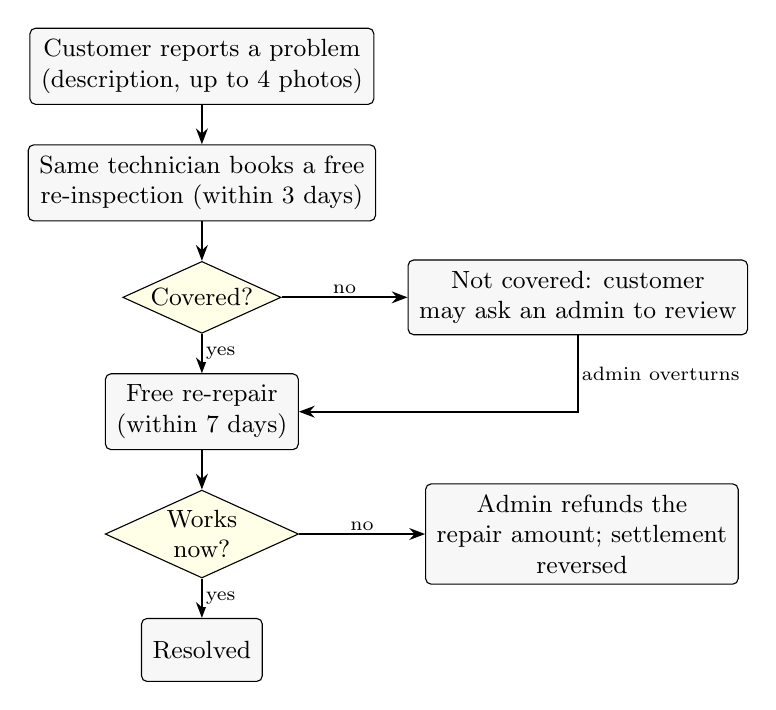
\begin{tikzpicture}[node distance=5mm and 8mm,font=\small]
  \node[box] (a) {Customer reports a problem\\(description, up to 4 photos)};
  \node[box,below=of a] (b) {Same technician books a free\\re-inspection (within 3 days)};
  \node[dec,below=of b] (c) {Covered?};
  \node[box,below=of c] (d) {Free re-repair\\(within 7 days)};
  \node[dec,below=of d] (e) {Works\\now?};
  \node[box,below=of e] (f) {Resolved};
  \node[box,right=16mm of c] (n) {Not covered: customer\\may ask an admin to review};
  \node[box,right=16mm of e] (r) {Admin refunds the\\repair amount; settlement\\reversed};
  \draw[arr] (a)--(b); \draw[arr] (b)--(c);
  \draw[arr] (c)--node[lbl,right]{yes}(d); \draw[arr] (c)--node[lbl,above]{no}(n);
  \draw[arr] (d)--(e); \draw[arr] (e)--node[lbl,right]{yes}(f); \draw[arr] (e)--node[lbl,above]{no}(r);
  \draw[arr] (n.south) -- node[lbl,right]{admin overturns} (n.south |- d.east) -- (d.east);
\end{tikzpicture}
\caption{Warranty claim lifecycle}
\label{fig:warranty}
\end{figure}

A customer may have one open claim at a time and at most two per repair. Every step is a guarded database update, so no step can be skipped and two people acting at once cannot both succeed. If the technician misses a deadline, the claim is marked overdue, admins are alerted and can take it over, and a technician with open claims cannot be removed. A refund covers the whole quote (repair payment plus the credited inspection fee) through Stripe with one idempotency key per part, so a retry never refunds twice. The technician's settlement for that repair becomes \emph{reversed}; if it had already been withdrawn, the wallet shows the amount as owed and it is deducted from future earnings. Figures~\ref{fig:scr-c16-warranty-claim}--\ref{fig:scr-c17-warranty-resolved} show a complete claim.

\section{Settlement and Withdrawal Lifecycle}
\begin{figure}[htbp]
\centering
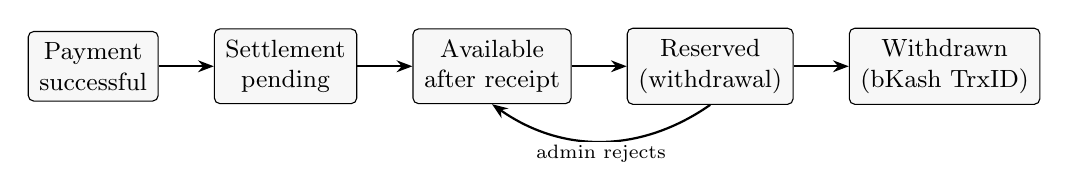
\begin{tikzpicture}[node distance=7mm,font=\small]
  \node[box] (a) {Payment\\successful};
  \node[box,right=of a] (b) {Settlement\\pending};
  \node[box,right=of b] (c) {Available\\after receipt};
  \node[box,right=of c] (d) {Reserved\\(withdrawal)};
  \node[box,right=of d] (e) {Withdrawn\\(bKash TrxID)};
  \draw[arr] (a)--(b); \draw[arr] (b)--(c); \draw[arr] (c)--(d); \draw[arr] (d)--(e);
  \draw[arr] (d.south) to[bend left=35] node[lbl,below]{admin rejects} (c.south);
\end{tikzpicture}
\caption{Technician settlement and withdrawal lifecycle}
\label{fig:settlement}
\end{figure}

The wallet is computed, not stored:
\begin{align}
\text{Pending} &= \textstyle\sum \text{paid settlements not yet receipt-confirmed}\\
\text{Gross available} &= \textstyle\sum \text{receipt-confirmed settlements} + \textstyle\sum \text{kept inspection-fee shares}\\
\text{Reserved} &= \textstyle\sum \text{open withdrawal requests}\\
\text{Withdrawn} &= \textstyle\sum \text{paid withdrawals}\\
\text{Available} &= \text{Gross available} - \text{Reserved} - \text{Withdrawn}
\end{align}
Because rejection simply removes a reservation, no compensating balance write is ever needed.

\paragraph*{Final payout when a technician is removed.}
\label{sec:removalpayout}
When an admin removes an approved technician, their whole available balance is queued as a withdrawal to their bKash number in the same database transaction as the removal, so either both happen or neither does. The number is taken, in order, from the admin's entry in the removal dialog, an already-open request (which is topped up rather than duplicated), the technician's last withdrawal, or their application phone. If money is owed and no valid number exists, the removal is refused until the admin enters one. Pending money is not yet available, so it is not included. The payout is tagged as a final payout in the admin queue and is sent and recorded with a bKash TrxID like any other withdrawal. Sarabo has no bKash API, so the transfer itself remains a manual bKash Send Money.

\section{Cancellation Rules}
Before a technician is booked, a customer can cancel a request freely; a cancelled request can be requested again with its details pre-filled. After booking with a paid fee, \texttt{GET /repair-requests/:id/booking-cancellation} tells the customer in advance which outcome cancelling now would have (refund or kept fee), and the cancellation itself is allowed only until the device is collected.

\section{Technician Profile Editing}
A technician can change their own name, phone, address and service area (region and district together) from the profile page; email, national ID, approval status and availability cannot be changed this way. The service area is locked while a repair is active, because the pickup was booked in the old area, and after a change the technician is told about open jobs in the new area.

\section{Service-Area Map}
\label{sec:areamap}
The public Service Areas page draws every listed district on an OpenStreetMap map (Leaflet) from the same \texttt{serviceAreas.json} file that drives the request form. Each district also stores the coordinates of its covered sub-areas. These were looked up once, offline, from OpenStreetMap and kept only if they lie inside that district (226 of 236). A search lists matching sub-areas before districts, so ``Ambarkhana'' opens Ambarkhana in Sylhet at street level instead of the city centre. A sub-area without a stored point falls back to its district's pin, and nothing is geocoded in the browser.

\section{Feedback and Moderation}
After a completed and receipt-confirmed repair, the customer may leave one review: a rating from 1 to 5 and an optional comment (up to 1,000 characters, plain text). Reviews are visible by default and admins can hide or restore them with a reason; every change is versioned and kept in a moderation history. Separately, a customer can file a private report about a technician (for example unprofessional behaviour, device damage or a payment issue). Reports go only to admins, move through \emph{open}, \emph{under review}, \emph{resolved} or \emph{dismissed}, and are never deleted with the request. Technicians see their average rating and visible reviews, but never reports or the reviewer's identity.

\section{Notifications and Reminders}
Forty-seven notification types, all defined in one module (\texttt{utils/notificationEvents.js}), cover offers, booking, refunds, inspection, quotes, payment, repair milestones, returns and disputes, warranty, reviews, withdrawals and a removed technician's final payout. Each has a de-duplication key. The daily job sends ``pickup tomorrow'' reminders in the app (and by email when enabled), once per pickup slot.

\section{Damage Image Upload}
\begin{figure}[htbp]
\centering
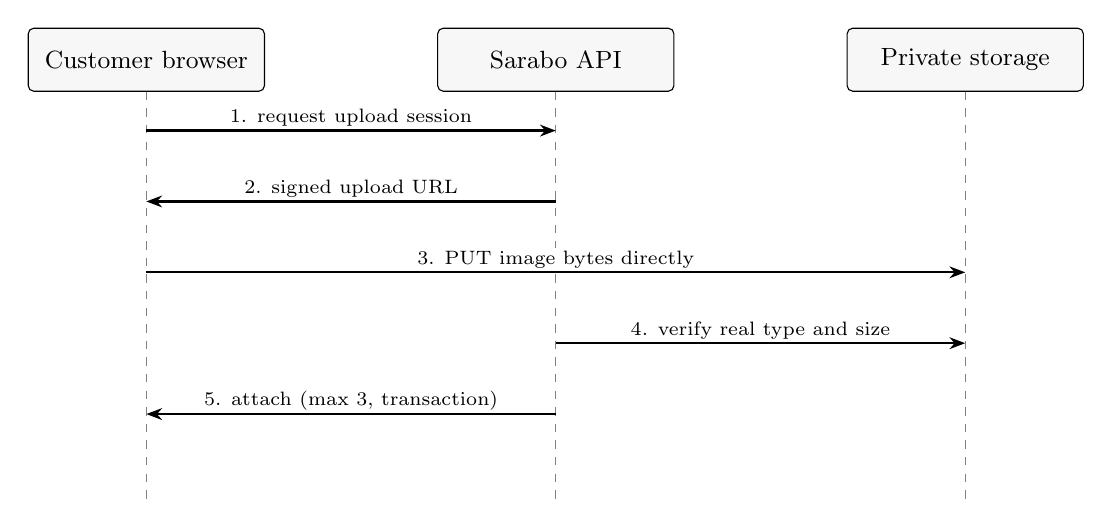
\begin{tikzpicture}[font=\small]
  \node[box,minimum width=3cm] (c) at (0,0) {Customer browser};
  \node[box,minimum width=3cm] (s) at (5.2,0) {Sarabo API};
  \node[box,minimum width=3cm] (st) at (10.4,0) {Private storage};
  \foreach \n in {c,s,st} \draw[dashed,gray] (\n.south) -- ++(0,-5.2);
  \draw[arr] (0,-0.9) -- node[lbl,above]{1. request upload session} (5.2,-0.9);
  \draw[arr] (5.2,-1.8) -- node[lbl,above]{2. signed upload URL} (0,-1.8);
  \draw[arr] (0,-2.7) -- node[lbl,above]{3. PUT image bytes directly} (10.4,-2.7);
  \draw[arr] (5.2,-3.6) -- node[lbl,above]{4. verify real type and size} (10.4,-3.6);
  \draw[arr] (5.2,-4.5) -- node[lbl,above]{5. attach (max 3, transaction)} (0,-4.5);
\end{tikzpicture}
\caption{Damage-image upload workflow}
\label{fig:upload}
\end{figure}

\end{document}
      % Chapter 6 Core Workflows and Business Rules
\documentclass{standalone}
\usepackage{standalone}

\begin{document}
\chapter{System Walkthrough}
\label{ch:walkthrough}

This chapter shows the running system. All screenshots were taken on 14 October 2026 from the final code, running locally with the development database, real Firebase sign-in, real Gemini answers and Stripe in test mode. Sections~\ref{sec:wt-request} to \ref{sec:wt-warranty} follow \emph{one} repair from start to finish (a Samsung Galaxy A54 with a cracked screen), switching between the customer's and the technician's screens as the case moves on, so every state in Figure~\ref{fig:e2e} appears in order. Other requests, technicians and figures visible in the lists come from the seeded development data.

\section{Public Website}
Anyone can see the services, prices, service areas, open jobs and the public tracking page without an account, and the AI support chat is available on every page.

\screen{p01-home}{Home page. The main actions are finding a repair service and tracking a repair; ``Ask Sarabo'' opens the AI support chat.}

\screen{p02-services}{Services and prices: the live catalogue of 45 services with their estimate ranges and inspection fees.}

\screen{p03-areas-search}{Service areas: searching ``Ambarkhana'' zooms the OpenStreetMap map to that sub-area of Sylhet and lists the other covered areas (Section~\ref{sec:areamap}).}

\screen{p05-ai-chat}{AI support chat answering a real question. The price and the 200\,BDT inspection fee come from the live catalogue, and the suggested buttons come from a fixed list (Chapter~\ref{ch:ai}).}

\screen{p04-jobs}{Public jobs board. Visitors see a safe summary of each open job (device, repair, area, pickup day, usual price, number of offers) but no customer details.}

\screen{p06-tracking}{Public tracking page for the walkthrough repair. Only the stage and its time stamps are shown; personal and payment details stay hidden.}

\begin{figure}[H]
\centering
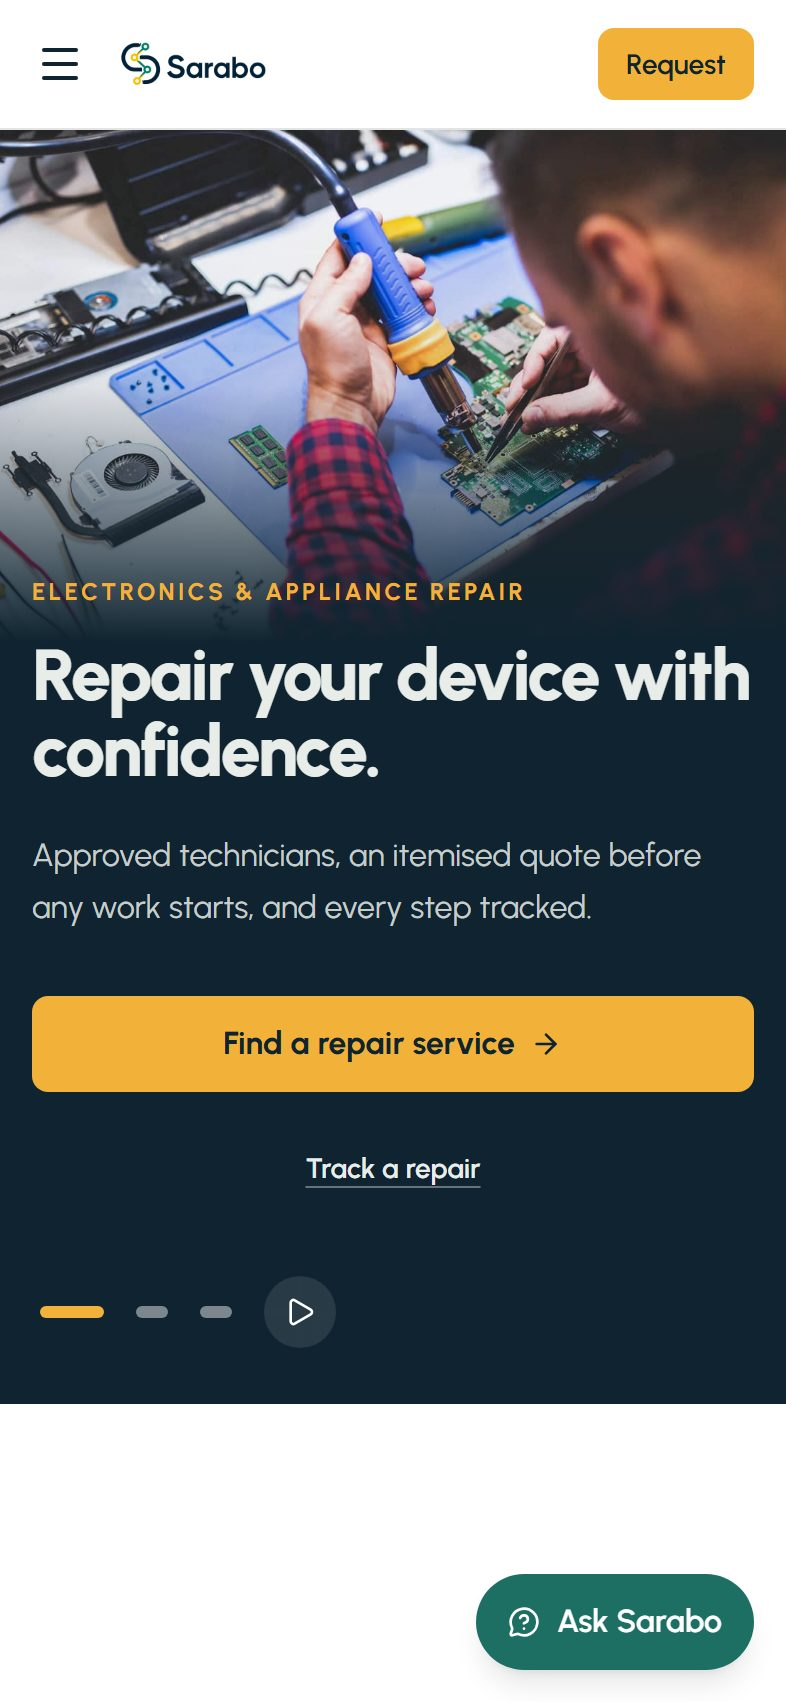
\includegraphics[width=0.34\textwidth]{img/screens/p08-mob-home}\hspace{8mm}
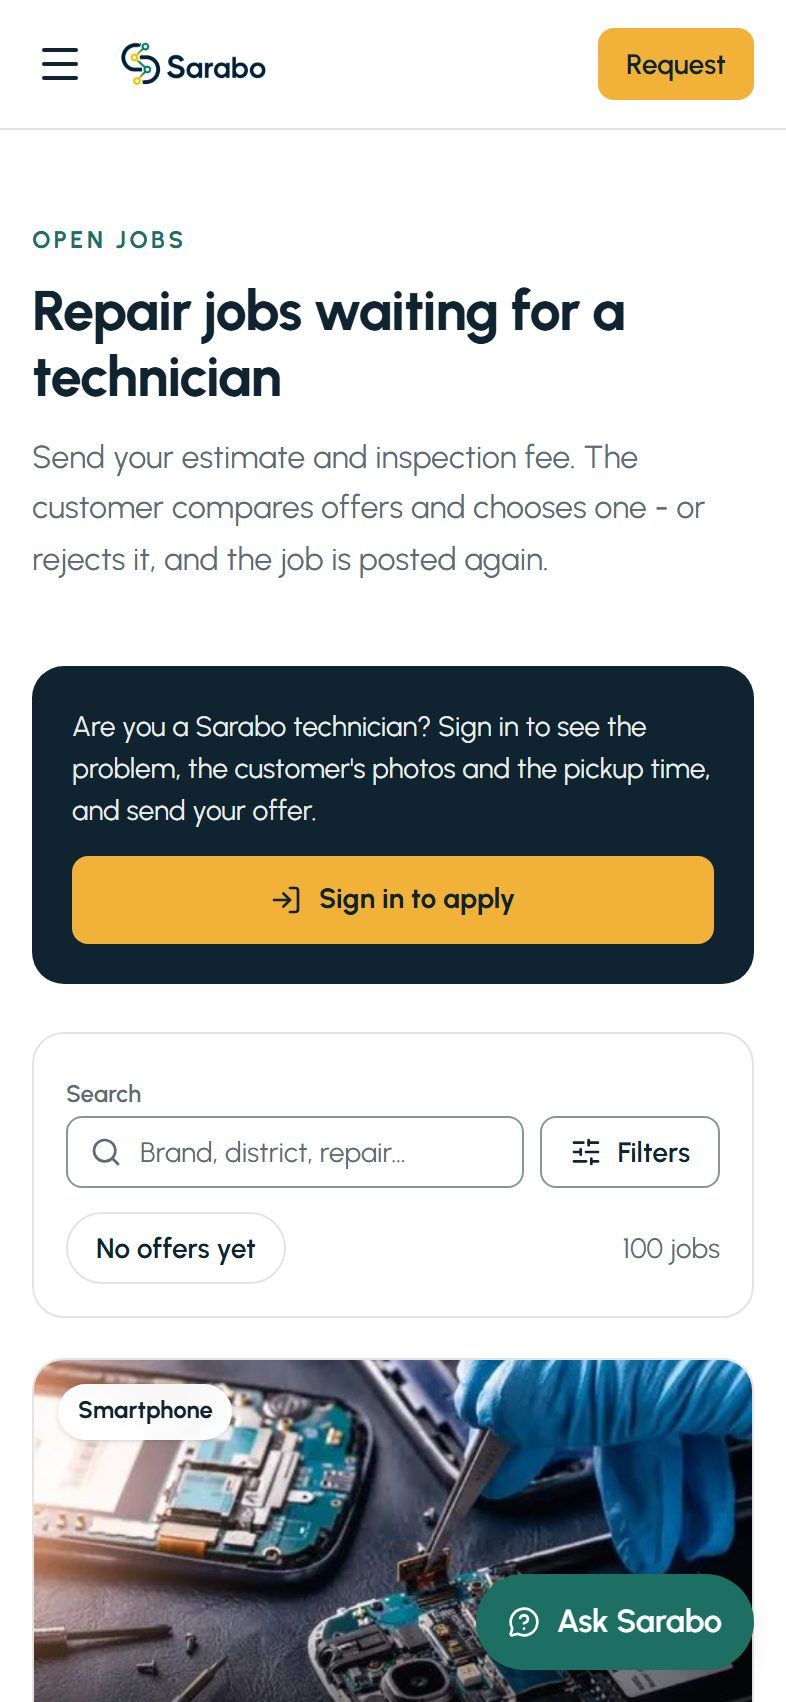
\includegraphics[width=0.34\textwidth]{img/screens/p09-mob-jobs}
\caption{The same pages on a phone (393\,px wide): home page and jobs board.}
\label{fig:scr-mobile}
\end{figure}

\section{Customer: Creating a Request}
\label{sec:wt-request}

\screen{c01-overview}{Customer overview: requests that need the customer first, then requests in progress.}

\screen{c02-ai-helper}{AI request helper. The customer wrote in Banglish (``\textit{Amar Samsung Galaxy A54 phone hat theke pore giye screen fete geche\ldots}''); Gemini filled in the device, brand, model, the catalogue service ``Screen Replacement'' and a clear English description. The summary on the right shows the estimate, and \emph{Undo} restores the form.}

\screen{c03-location-pickup}{Location and pickup window: region, district, address, then a two-hour slot (Saturday--Thursday, Friday closed).}

\screen{c04-created}{Request created. The customer can add up to three damage photos now or later; photos are sent only when the customer presses ``Upload''.}

\section{Technician: Finding the Job and Sending an Offer}

\screen{t02-jobs}{Jobs board for a signed-in technician, with filters for region, device, repair, ``No offers yet'', ``Not applied'' and ``My offers''.}

\screen{t03-offer}{Sending an offer. The price guide (top) shows what technicians usually offer for this repair. The fee field enforces the minimum inspection fee (200\,BDT here). The technician typed only ``likely display panel and touch, original screen available'', and \emph{Write it for me} turned it into the note.}

\section{Customer: Choosing a Technician and Booking}

\screen{c05-my-requests}{My repairs: the new request asks the customer to choose a technician because an offer is waiting.}

\screen{c06-offers}{Offer from a technician, with the ranking reasons from Section~\ref{sec:ranking}: ``12 repairs, no missed pickups'', ``In your district'' and ``Usually replies in 2 min'', plus rating, level, experience, estimate, fee and the AI-written note.}

\screen{c07-choose}{Choosing the offer: the customer pays the inspection fee to book the visit. The fee counts toward the final price and is refunded if the booking fails.}

\screen{c08-stripe}{Stripe Checkout (test mode, sandbox badge) for the 200\,BDT inspection fee, paid with Stripe's published test card.}

\screen{c09-booked}{After payment the technician is booked. The page confirms the fee and that it counts toward the final price; ``Cancel visit'' applies the cancellation rules in Table~\ref{tab:feeoutcomes}.}

\section{Technician: Pickup, Inspection and Quote}

\screen{t04-assigned}{Assigned jobs, with the next action (``Start pickup'') on each job.}

\screen{t05-pickup-condition}{Recording the device's condition and accessories at pickup (Section~\ref{sec:nostuck}). The customer sees this record and can dispute it.}

\screen{t06-inspection}{Inspection: findings, detected issues with severity, a repairability decision and a preliminary estimate. ``Not repairable'' or ``Not economical'' would let either side close the request.}

\screen{t07-quote}{Itemised quote: labour 800 + parts 3,200 = 4,000\,BDT. The form shows the 10\% platform commission and what the technician receives.}

\section{Customer: Approving the Quote and Paying}

\screen{c10-quote}{The customer reviews the quote. The 200\,BDT fee already paid is subtracted, so 3,800\,BDT is left to pay, and the approve button says so.}

\screen{c11-approve-pay}{``Approve and pay'' leads straight to the card payment.}

\screen{c12-payment-success}{Payment successful, with the Stripe transaction ID, the tracking code and a PDF receipt download.}

\screen{c13-payment-history}{Payment history: one row each for the 3,800\,BDT repair payment and the 200\,BDT inspection fee, each with a PDF receipt.}

\section{Technician: Repair and Hand-Over}

\screen{t08-progress}{Repair in progress: the technician posts progress updates that the customer sees.}

\screen{t09-complete}{Completing the repair with a summary of the work (and up to three optional completion photos). ``Can't finish this repair'' sends the case to an admin for a refund instead.}

\screen{t10-returned}{Marking the device returned. If the customer does not answer within three days, receipt is confirmed automatically.}

\section{Customer: Receipt, Review and Warranty}
\label{sec:wt-warranty}

\screen{c14-confirm-receipt}{The customer confirms receipt, or reports ``I haven't received it'', which goes to an admin. Confirming makes the technician's earning available and starts the warranty.}

\screen{c15-review}{Rating the technician (1--5 with an optional comment). A private report to admins is a separate action.}

\screen{c16-warranty-claim}{Reporting a problem under the 30-day warranty: the customer says what happened (same fault, or a fitted part failed), describes it and can add photos.}

\screen{t11-warranty-book}{The technician books the free re-inspection, which must happen within three days, otherwise an admin can take the claim over.}

\begin{figure}[H]
\centering
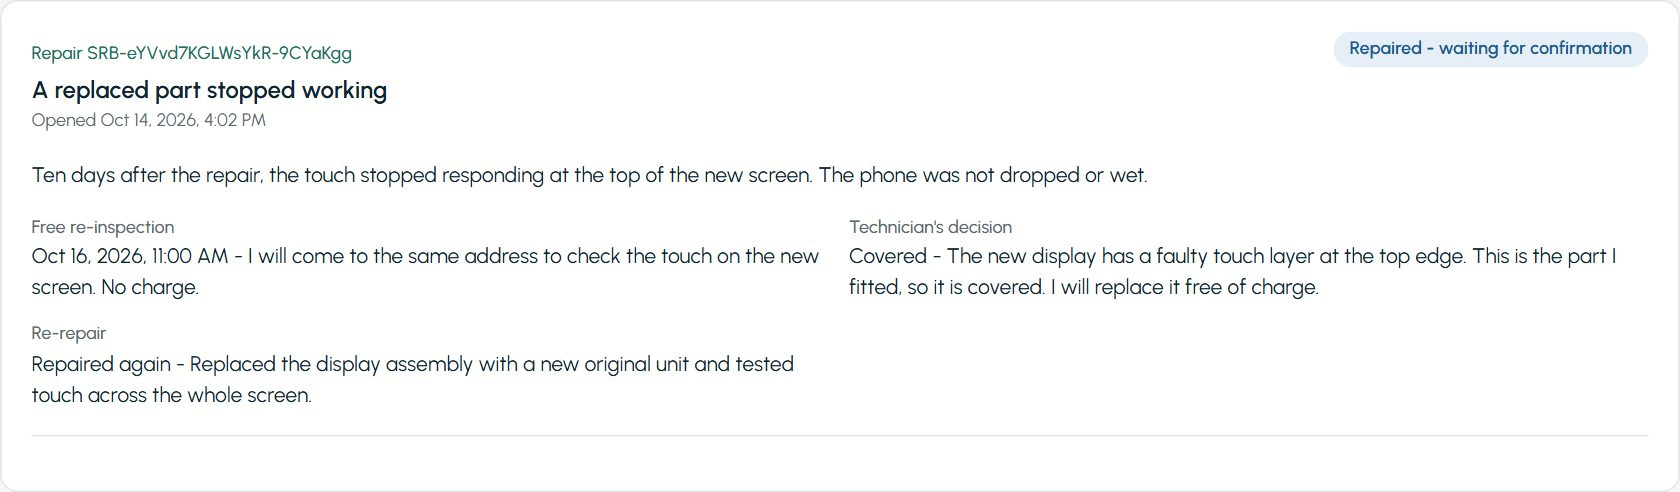
\includegraphics[width=0.92\textwidth]{img/screens/t12-warranty-card}
\caption{The technician's warranty claim after the visit: booked re-inspection, decision ``Covered'' and the re-repair, each with its note.}
\label{fig:scr-t12-warranty-card}
\end{figure}

\screen{c17-warranty-resolved}{The customer's view at the end: the claim shows every step and the customer's answer ``Working now'', so the claim is resolved. Had the re-repair failed, an admin would have refunded the repair.}

\screen{c18-notifications}{Customer notifications for every step of this repair.}

\section{Technician: Wallet, Profile and History}

\screen{t01-overview}{Technician overview: available balance, active jobs and rating.}

\screen{t13-wallet}{Wallet after this repair: the 3,600\,BDT earning (4,000 minus 10\%) requested as a bKash withdrawal, shown as ``Withdrawal in progress''. Balances are computed from settlements and withdrawals, never stored.}

\screen{t14-profile-edit}{Editing the technician's own details (name, phone, region, district, address). The area cannot change while a repair is active.}

\screen{t15-completed-jobs}{Completed jobs, each with the amount the technician receives.}

\section{Admin}

\screen{a01-overview}{Admin overview. The ``Needs you'' panel counts missed and overdue pickups, requests with no offers in 24 hours, stalled repairs and requests no local technician can take; each count opens its filtered list. (The counts come from the seeded development data.)}

\screen{a02-requests}{All repair requests, with search, status and payment filters and selectable columns.}

\screen{a03-request-detail}{The walkthrough repair from the admin's side, with the full record including the pickup condition.}

\screen{a04-assign}{Assign technicians: requests waiting for a technician, with flags such as ``Pickup time passed'' and ``No offers in 24h''. The admin can invite a technician to apply or assign one directly.}

\screen{a05-technicians}{Technician applications and approved technicians with their expertise, approval status and availability.}

\screen{a06-catalogue}{Services and prices: the catalogue editor, showing for each service its open requests.}

\screen{a07-service-editor}{Editing a service. Price changes create a new pricing version and never change existing requests; the inspection fee cannot be set below the minimum.}

\screen{a08-reports}{Reports with the AI summary. The model only sees aggregate figures, and any sentence with a number that is not in the facts is removed before saving.}

\begin{figure}[H]
\centering
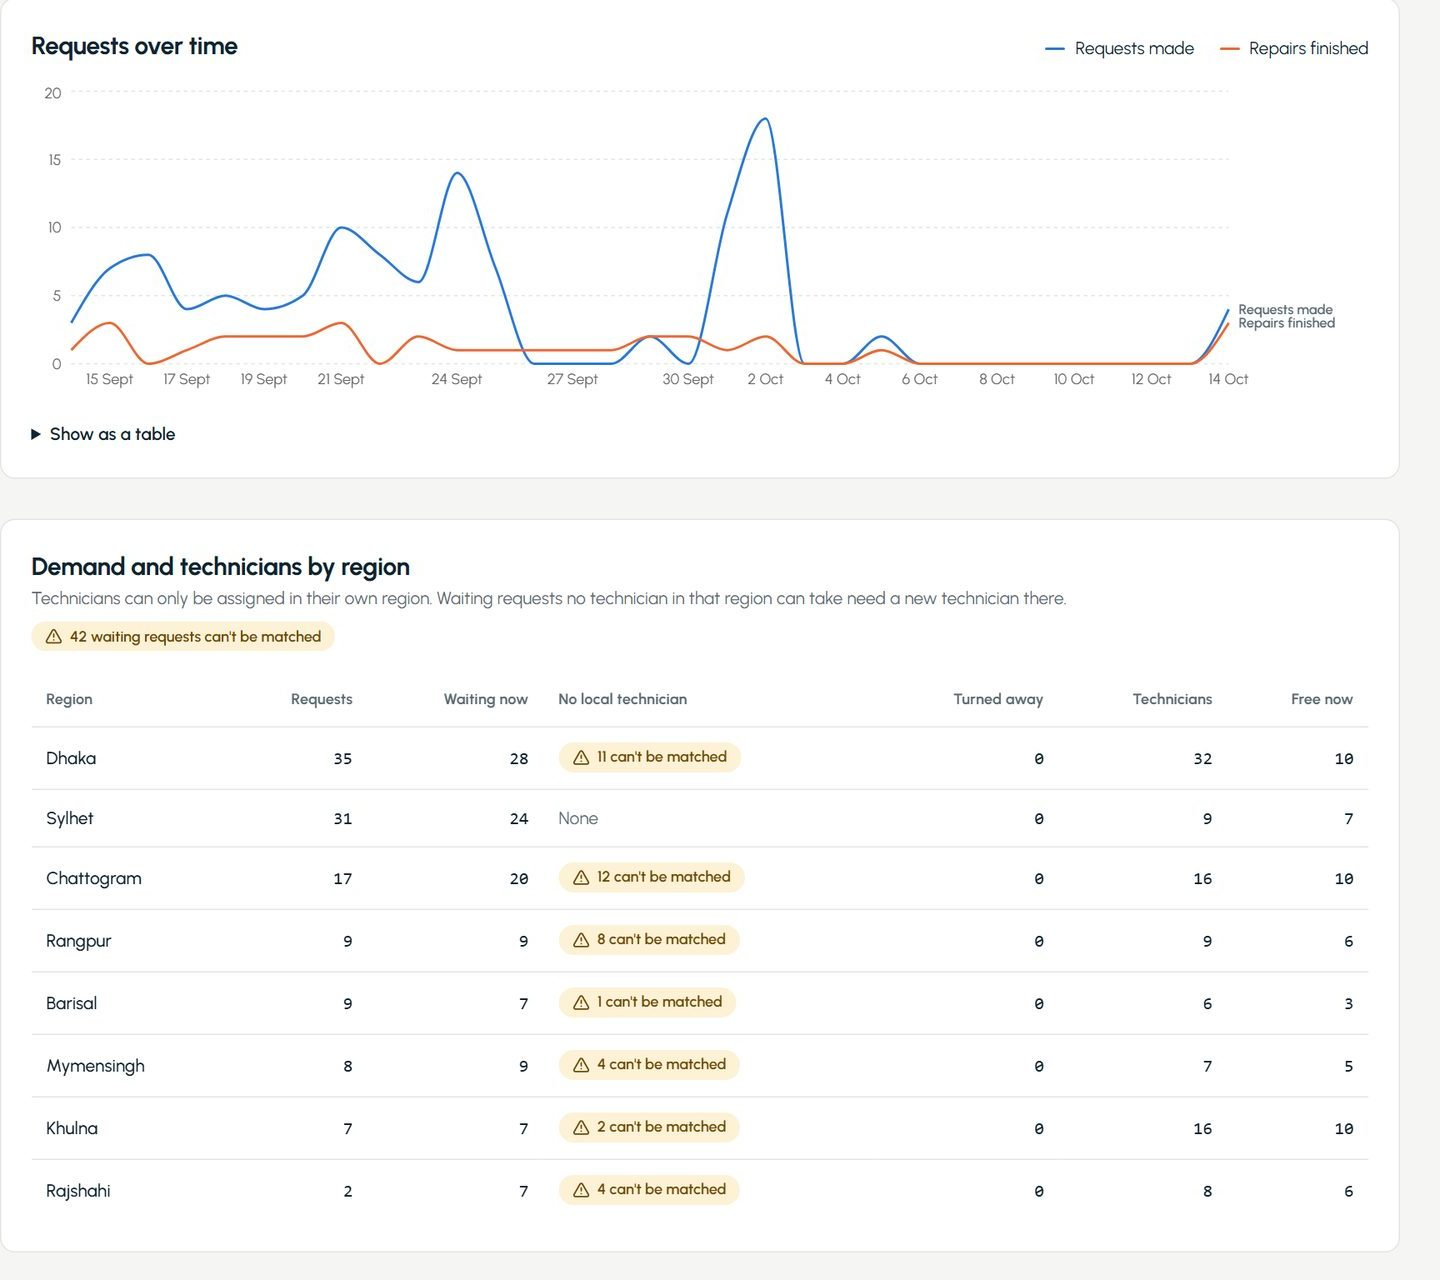
\includegraphics[width=0.48\textwidth]{img/screens/a09-reports-charts}\hfill
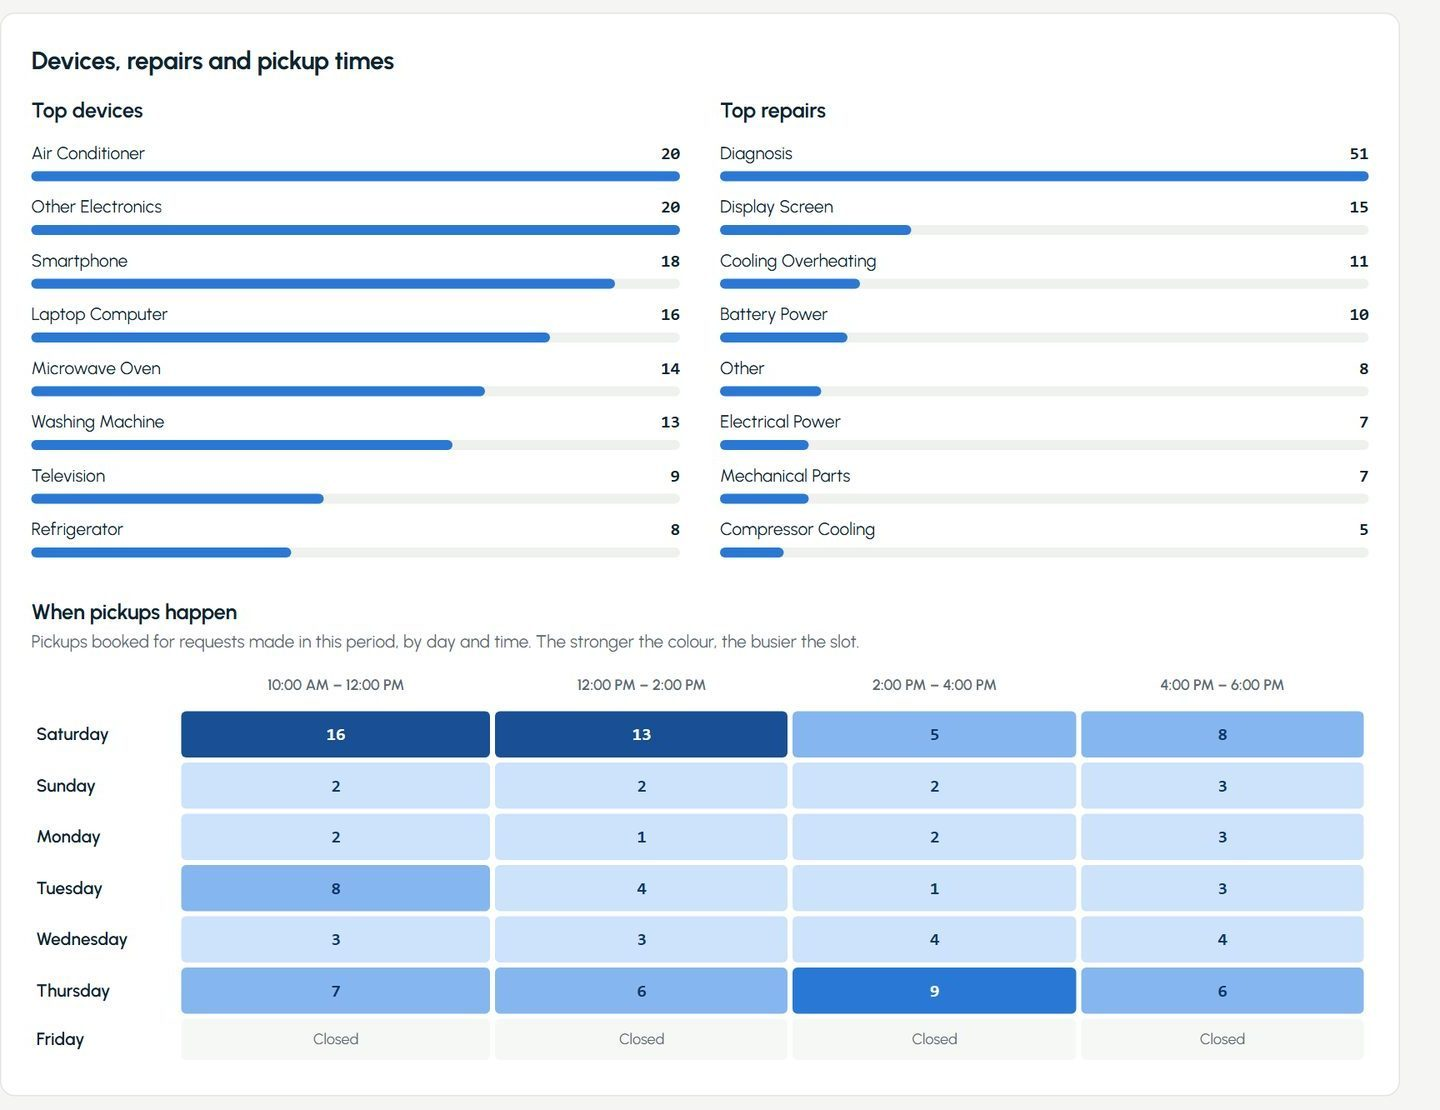
\includegraphics[width=0.48\textwidth]{img/screens/a09b-reports-charts2}
\caption{Report charts: requests over time and demand against technicians by region (left); top devices and repairs and a pickup heat map by day and time (right).}
\label{fig:scr-reports-charts}
\end{figure}

\screen{a10-mark-paid}{Recording a bKash payout. The admin sends the money with bKash Send Money first, then records the TrxID; this test record used a made-up TrxID.}

\screen{a11-reviews}{Technician reviews, including the walkthrough review. Admins can hide or restore a review with a reason, and every change is kept.}

\screen{a12-users}{User management: roles can be changed only by an admin.}

\end{document}
   % Chapter 7 System Walkthrough (screenshots)
\documentclass{standalone}
\usepackage{standalone}

\begin{document}
\chapter{AI-Assisted Features}
\label{ch:ai}

Sarabo uses Google Gemini in four places where it saves users real effort. In every case the AI \emph{suggests} and a person \emph{decides}: nothing the model returns changes a price, a payment or a request state without a human reviewing it first. All four features are switched off by default and need both an explicit setting and an API key; the client asks \texttt{GET /ai/status} and hides a feature that is not available. The model is \texttt{gemini-3.5-flash-lite}; if it is slow, overloaded or rate-limited, the same request goes to \texttt{gemini-3.1-flash-lite} as a fallback.

\section{AI Customer Support Chat}
A chat widget on every page answers visitor and customer questions about how Sarabo works, which services exist and what they usually cost. The prompt is built from the \emph{live} service catalogue (\texttt{supportKnowledgeService}), so answers about prices always reflect the current catalogue. Conversation history, message length and answer length are capped, and suggested follow-up buttons (View services, Track a request, Log in, Create an account) are chosen from a fixed list rather than generated as free links (Figure~\ref{fig:wt-p05}).

\section{AI Request Helper}
On the create-request form a customer can describe the problem in their own words (Bangla, English or the common mixed ``Banglish'') and/or add a photo of the damage. The AI returns a draft: device category, catalogue service, brand, model, a clear English description, a confidence level, an optional follow-up question and, when a photo was sent, whether it actually shows a device and what is visible. The form fills itself, the customer edits anything, and \emph{Undo} restores what was there before (Figure~\ref{fig:wt-c02}). If the photo shows a device, it is uploaded to the new request automatically after creation, so the customer does not have to pick it twice.

\section{Technician Price Guide and AI Offer Note}
When a technician writes an offer, a price guide (computed without AI) shows the usual range from real offers for the same service in the last 180 days: the 25th percentile of ``from'' prices to the 75th percentile of ``to'' prices, and the same for inspection fees. With fewer than three past offers it falls back to the catalogue range. The form gives advisory warnings if an offer is far outside the usual range.

The technician can also ask AI to write the offer note in English or Bangla. The model sees only what the technician already sees (device, brand, model, repair, the customer's problem text and whether photos exist), writes in the technician's voice, describes the likely issue only as a possibility, says the final price comes after inspection, and contains no numbers. Phone numbers (including Bangla digits), emails, links and social handles are stripped from the answer so that contact stays on the platform (Figure~\ref{fig:wt-t03}).

\section{AI Summary of Admin Reports}
The admin Reports page (7, 30 or 90 days) can show a short AI summary: a headline, two to four highlights and one to three suggested actions. The model receives only aggregate figures (requests made, finished and cancelled, success rate, average days, refused demand by region, top devices and repairs, technician workload, inspection-fee money and current attention counts), never names, emails or IDs. The last summary per period is stored, so opening the page costs nothing (Figure~\ref{fig:wt-a08}).

\section{Safeguards}
Table~\ref{tab:aisafety} summarises how the main risks of LLM features~\cite{owaspllm} are handled.

\begin{table}[htbp]
\centering
\caption{AI risks and safeguards}
\label{tab:aisafety}
\small
\begin{tabularx}{\textwidth}{@{}p{3.4cm}X@{}}
\toprule
\textbf{Risk} & \textbf{Safeguard in Sarabo} \\
\midrule
Invented catalogue items & The request helper must answer with IDs from an enum built from the live catalogue (JSON schema); the server re-checks them and drops unknown or inactive IDs, or a repair belonging to another device. \\
Invented prices & No AI feature ever sets a price. Estimates come from the catalogue; the offer note contains no numbers. \\
Invented statistics & Every sentence of the report summary is checked: each number must appear in the facts, be a difference or rounded percentage between periods, a small count up to 10, or a fixed context number. Failing sentences are dropped; if nothing remains, the request fails with 502. \\
Prompt injection & Customer text is marked as untrusted data in the prompt, and output is forced into a schema. \\
Personal data leakage & Text containing a card number, password, token or tracking code is refused before any AI call. Models receive no names, emails or addresses. Contact details are stripped from generated notes. \\
Unbounded cost & Per-user 10-minute and daily limits plus a site-wide daily budget per feature, stored in MongoDB so all serverless instances share them. If the database is unreachable, the feature fails closed. \\
Bad photos & JPEG/PNG/WebP only, at most 1.5\,MB, first bytes must match the type; the client shrinks photos to 1024\,px first. The helper's photo is not stored by the AI endpoint. \\
Provider failure & If the first model is slow (over 5\,s for support), overloaded or rate-limited, the request goes straight to the fallback model; otherwise controlled errors (503 unavailable, 504 timeout, 502 invalid answer) and the rest of the form keeps working. Live support answers take 1.4--1.9\,s. \\
\bottomrule
\end{tabularx}
\end{table}

\begin{table}[htbp]
\centering
\caption{Default AI usage limits}
\label{tab:ailimits}
\small
\begin{tabular}{@{}lccc@{}}
\toprule
\textbf{Feature} & \textbf{Per user / 10 min} & \textbf{Per user / day} & \textbf{Site / day} \\
\midrule
Support chat (signed in) & 20 & 100 & 300 \\
Support chat (anonymous) & 8 & 30 & (shared) \\
Request helper & 10 & 30 & 200 \\
Offer note & 10 & 40 & 200 \\
Report summary & 5 & 20 & 50 \\
\bottomrule
\end{tabular}
\end{table}

All AI tests use fake providers, so the automated suites never call Gemini or spend money.

\end{document}
      % Chapter 8 AI-Assisted Features
\documentclass{standalone}
\usepackage{standalone}

\begin{document}
\chapter{Security, Reliability and Data Integrity}

\section{Security Principles}
Sarabo is \emph{server-authoritative}. The client decides what to display; the server decides what is allowed. This follows the common REST security guidance that authorization must be enforced at each resource operation~\cite{owasprest}. Secrets (database, Stripe, Supabase, Gemini, Gmail, cron) exist only in server environment variables and are never committed or sent to the browser.

\section{Authentication}
Firebase issues ID tokens to signed-in users. Each protected request sends the token, the server verifies it with Firebase Admin, and the caller's email is taken from the verified token only. Endpoints such as \texttt{/technicians/me}, \texttt{/users/me/role} and the wallet never accept another user's email as input. Customer actions that create requests or payments require a verified email address.

\section{Role- and State-Based Authorization}
Every write endpoint checks both who the caller is and what state the request is in:
\begin{itemize}
  \item only Admins approve technicians, edit the catalogue, retry refunds, process withdrawals and moderate feedback;
  \item only an approved, matching Technician can see job details or send an offer, and only the booked Technician can inspect, quote, revise and repair;
  \item only the owning Customer can choose or reject offers, decide on a quote, pay, cancel, confirm receipt and review;
  \item a quote can be submitted only after inspection, payment only after approval, revision only from \texttt{quote\_rejected}, and a paid repair can never re-enter the rejected-quote path.
\end{itemize}
Requests that do not belong to the caller return the same ``not found'' answer as missing ones, so their existence is not revealed.

\section{Financial Integrity}
Prices, fees, credits, commissions, balances and withdrawal limits are always derived on the server from stored data. Money is handled in whole taka. Stripe sessions are created from stored amounts; the webhook signature is verified on the raw body~\cite{stripewebhooks}; payment processing is idempotent; refunds carry idempotency keys; settlements are frozen once; and withdrawals move from \emph{requested} to \emph{paid} or \emph{rejected} through a single-winner update, so the same withdrawal can never be paid twice.

\section{Privacy}
Public endpoints (tracking, jobs board, service availability) return purpose-built projections without names, emails, addresses, phone numbers, payment data or database IDs. Technicians see a customer's district and problem, but not identity or street address, until booked. Refused-demand counts store a hash instead of the customer's email. Reports about technicians are visible only to admins.

\section{Private Image Security}
The storage bucket is private. Signed upload and read URLs are short-lived and specific to one object. The server checks the real stored type and size rather than trusting the browser, and the permanent object identifier is never returned by the API.

\section{Input Validation and Safe Errors}
The server validates IDs, state transitions, amounts, text lengths, file types and every mutation's allowed fields; unexpected fields are rejected. User text is stored as plain text and rendered as text. Errors use stable codes (for example \texttt{PICKUP\_SLOT\_FULL}, \texttt{NO\_TECHNICIAN\_AVAILABLE}) instead of raw provider messages, and logs record only the request ID, route, status and a broad category, never request bodies, comments or secrets.

\section{CORS, Rate Limiting and Abuse Control}
The API accepts browser calls only from the configured client origin, which must be \texttt{https} in production. Public tracking, the jobs board and every AI feature are rate limited; AI and support limits are stored in MongoDB so they hold across serverless instances. The scheduled job endpoint requires a secret and refuses to run without one.

\section{Transaction Safety}
MongoDB transactions protect the invariants that matter most:
\begin{itemize}
  \item a request's state and its technician's availability always agree, so a technician cannot be double-booked;
  \item a payment, the booking it causes and the offers it closes change together;
  \item a quote transition, its tracking event and its notification apply together or not at all;
  \item a fee refund is marked pending in the same transaction as the event that causes it.
\end{itemize}
A late defect (Appendix~\ref{app:incident}) showed a subtle rule: if an insert inside a transaction fails with a duplicate key, MongoDB has already aborted the transaction, so that error must be passed on to let the driver retry the whole transaction, never swallowed.

\section{Environment Isolation}
Development, automated tests and production use different database names, and the code refuses to run tests against the development or production database. Seed and migration scripts default to dry runs and refuse production unless an operator passes explicit one-time flags. Continuous integration runs on a throwaway database and is never given real credentials.

\section{Legacy Compatibility Boundary}
Some stored values come from the original parcel-delivery codebase: the role value \texttt{rider} and status values such as \texttt{driver\_assigned} or \texttt{parcel\_delivered}. They are treated as frozen contract values behind a presentation layer; everything users see uses repair terminology. Renaming them would require a coordinated data migration and is listed as future work.

\end{document}
      % Chapter 9 Security, Reliability and Data Integrity
\documentclass{standalone}
\usepackage{standalone}

\begin{document}
\chapter{Testing and Evaluation}
\label{ch:testing}

\section{Testing Strategy}
Testing focused on \emph{domain correctness}: whether the right person can do the right thing at the right time, exactly once. Four layers were used (Figure~\ref{fig:testlayers}).

\begin{figure}[htbp]
\centering
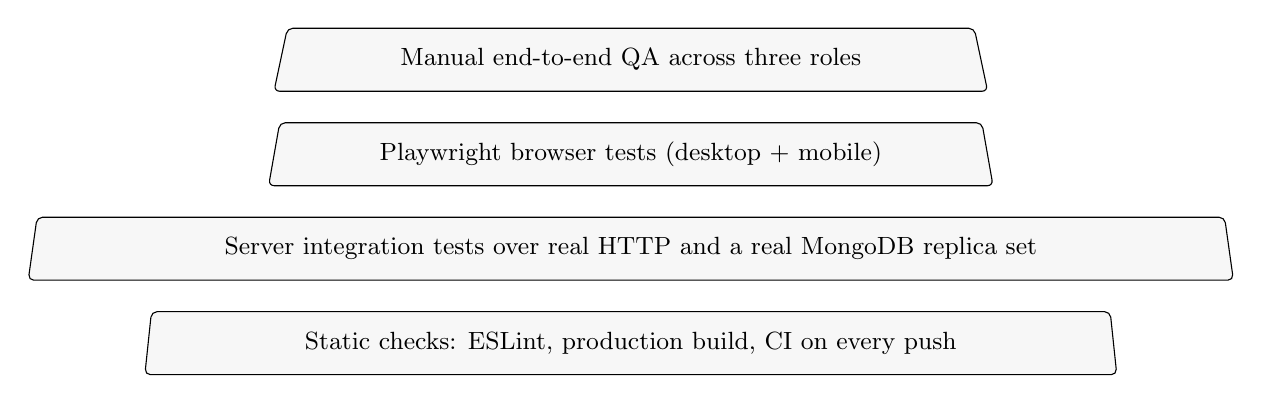
\begin{tikzpicture}[font=\small]
  \node[box,trapezium,trapezium angle=78,minimum width=6cm] (a) at (0,2.4) {Manual end-to-end QA across three roles};
  \node[box,trapezium,trapezium angle=80,minimum width=8cm] (b) at (0,1.2) {Playwright browser tests (desktop + mobile)};
  \node[box,trapezium,trapezium angle=82,minimum width=10cm] (c) at (0,0) {Server integration tests over real HTTP and a real MongoDB replica set};
  \node[box,trapezium,trapezium angle=84,minimum width=12cm] (d) at (0,-1.2) {Static checks: ESLint, production build, CI on every push};
\end{tikzpicture}
\caption{Testing layers used in Sarabo}
\label{fig:testlayers}
\end{figure}

\paragraph*{Server integration tests.} A custom harness (\texttt{test-all.js}) starts its own API server on a random port against an isolated test database, seeds a baseline (role accounts, an approved technician, the catalogue) and exercises endpoints over real HTTP, plus direct service-level checks. Stripe, Supabase, Gemini and email are replaced by injected fakes, so the suite never touches external services or money. Concurrency is tested by firing competing requests at once, for example two admins assigning different technicians to the same request, a cancellation racing a payment, or the same Stripe webhook delivered several times in parallel; each must produce exactly one winner and a consistent final state.

\paragraph*{Browser tests.} Playwright runs against a real production build of the client with a faked API, on a desktop and a mobile (Pixel~7) viewport. The tests cover public pages, the jobs board (listing, filtering, sorting, empty and error states), tracking (valid, unknown, invalid codes and server errors), authentication forms and route protection.

\paragraph*{Continuous integration.} GitHub Actions runs the server suites against a throwaway MongoDB~8 replica set and runs client lint and build on every push and pull request. The latest runs on the main branch of both repositories (11 October 2026, on the final commits) passed.

\section{Verification Results}
\label{sec:results}
For this report every check was run again on 11 October 2026 against the final code (client commit \texttt{428ee11}, server commit \texttt{0d1e758}). The server suites were run exactly as in CI, using a clean copy of the repository with no local secrets and a temporary in-memory MongoDB replica set. Table~\ref{tab:results} shows the results.

\begin{table}[htbp]
\centering
\caption{Verification results (11 October 2026)}
\label{tab:results}
\small
\begin{tabularx}{\textwidth}{@{}Xrr@{}}
\toprule
\textbf{Check} & \textbf{Passed} & \textbf{Failed} \\
\midrule
Server full suite (\texttt{npm test}) & 2,595 & 0 \\
\quad of which re-run on their own: support and AI suite & 160 & 0 \\
\quad of which re-run on their own: data-migration suite & 63 & 0 \\
\quad of which re-run on their own: feedback suite & 177 & 0 \\
Client browser tests (Playwright, 29 scenarios $\times$ 2 viewports) & 58 & 0 \\
Client ESLint & \multicolumn{2}{r}{no errors} \\
Client production build & \multicolumn{2}{r}{success} \\
GitHub Actions, latest \texttt{main} run, both repositories & \multicolumn{2}{r}{success} \\
\bottomrule
\end{tabularx}
\end{table}

The server suite has grown from 1,890 checks at the time of the earlier report (August 2026) to 2,595, mainly through coverage of the job portal, inspection-fee outcomes, pickup scheduling, email, reports and the AI features. The last 15 of these cover the final payout on technician removal.

\section{Representative Test Scenarios}
\begin{longtable}{@{}p{1.1cm}p{6.1cm}p{6.9cm}@{}}
\caption{Representative test scenarios}\label{tab:scenarios}\\
\toprule
\textbf{ID} & \textbf{Scenario} & \textbf{Expected and verified result} \\
\midrule
\endfirsthead
\toprule
\textbf{ID} & \textbf{Scenario} & \textbf{Expected and verified result} \\
\midrule
\endhead
\bottomrule
\endfoot
T-01 & Request without a token to a protected endpoint & 401; no data returned \\
T-02 & Customer calls an admin endpoint & 403; nothing changes \\
T-03 & Request in a region with no matching technician & 409 \texttt{NO\_TECHNICIAN\_AVAILABLE}; refusal counted once per day \\
T-04 & Customer picks a pickup slot that is already full & 409 \texttt{PICKUP\_SLOT\_FULL}; request not saved \\
T-05 & Unapproved or non-matching technician sends an offer & Refused; offer not stored \\
T-06 & Inspection fee above the catalogue cap & Refused by the server \\
T-07 & Fee payment arrives after another technician was booked & Payment recorded and refunded automatically \\
T-08 & Same Stripe event delivered twice, or webhook and success page both fire & Exactly one payment row and one booking \\
T-09 & Customer rejects an offer & Job reposted; technician may send one revised offer only \\
T-10 & Cancel 3 hours vs 1 hour before pickup & Full refund vs fee kept and split 90/10 \\
T-11 & Stripe refund call fails & Refund stays pending, shows on admin home, retry succeeds once \\
T-12 & Quote submitted before inspection & Controlled conflict; state unchanged \\
T-13 & Quote rejected, revised and resubmitted & Old quote archived; new round gets its own notification; no transaction hang \\
T-14 & Approved quote with fee already paid & Amount due = quote total minus fee; settlement on the full quote \\
T-15 & Paid request moves on to repair states & Still reported as paid; no second Pay button \\
T-16 & Repair completed but not yet received & Settlement pending; cannot be withdrawn \\
T-17 & Withdrawal above available balance, or two open withdrawals & Refused; database allows only one open request \\
T-18 & Withdrawal marked paid, then technician asks again & Nothing left to withdraw; balance can never go negative \\
T-19 & Duplicate review, or review before receipt & Refused; one review per repair \\
T-20 & AI draft names an unknown or inactive service & ID dropped by the server \\
T-21 & AI summary sentence with a number not in the facts & Sentence removed before saving \\
T-22 & Problem text containing a card number & Refused before any AI call \\
T-23 & Public tracking and jobs board responses & No names, emails, addresses or payment data \\
T-24 & Seed or migration script pointed at production & Refused without explicit operator override \\
T-25 & Admin removes a technician with 3,000 BDT available & Removal and a 3,000 BDT final bKash withdrawal commit together; with no bKash number on record, removal is refused and nothing changes \\
T-26 & Visitor searches ``Ambarkhana'' on the Service Areas page & Map zooms to Ambarkhana in Sylhet, not the district centre; ``Sylhet'' still opens the district \\
\end{longtable}

\section{Manual End-to-End Acceptance}
In August 2026 the core lifecycle was accepted by hand in the development environment with three accounts and Stripe test cards: request, assign, accept, inspect, quote, reject, revise, re-quote, approve, pay, repair, complete and confirm receipt, checking at each step that all three roles saw the same state and that the settlement became available only after receipt. For the final submission the same walkthrough is extended to the marketplace flow (AI-assisted request, offers, offer rejection and repost, inspection-fee payment, approve-and-pay, bKash withdrawal and review) as part of the final improvement phase (Section~\ref{sec:finalphase}).

\section{Evaluation Against Objectives}
\begin{table}[htbp]
\centering
\caption{Evaluation against objectives}
\label{tab:evaluation}
\small
\begin{tabularx}{\textwidth}{@{}p{1cm}p{1.8cm}X@{}}
\toprule
\textbf{Obj.} & \textbf{Status} & \textbf{Evidence} \\
\midrule
O1 & Achieved & Firebase identity, server role and state checks (T-01, T-02) \\
O2 & Achieved & Structured V2 form, catalogue, photos, pickup slots, AI helper (T-04, T-20) \\
O3 & Achieved & Region and expertise gate, jobs board, offers and reposting (T-03, T-05, T-09) \\
O4 & Achieved & Fee booking, credit, refunds and split (T-06, T-07, T-10, T-11, T-14) \\
O5 & Achieved & Inspection, quote, rejection and revision (T-12, T-13) \\
O6 & Achieved & Single payment truth, idempotent processing, PDF receipts (T-08, T-15) \\
O7 & Achieved & Progress, evidence, receipt confirmation, reviews and reports (T-16, T-19) \\
O8 & Achieved & 41 notification types, email, daily reminders, sanitized tracking (T-23) \\
O9 & Achieved & 90/10 settlement, computed wallet, bKash withdrawals, final payout on removal (T-16 -- T-18, T-25) \\
O10 & Achieved & Attention list, reports with checked AI summary, catalogue editor, moderation (T-21) \\
O11 & Achieved & 2,595 server checks, 58 browser tests, lint, build, CI, live deployment \\
\bottomrule
\end{tabularx}
\end{table}

\section{Validation Boundary}
The automated results above refer to an isolated test environment with fake external providers. Payments run in Stripe test mode, so no real money has moved through the platform, and the system has not yet been used by real customers. Load and performance testing under heavy traffic, and a formal security audit, were outside the scope of this project.

\end{document}
      % Chapter 10 Testing and Evaluation
\documentclass{standalone}
\usepackage{standalone}

\begin{document}
\chapter{Limitations and Future Work}
\label{ch:limitations}

\section{Current Limitations}
\begin{itemize}
  \item \textbf{Technician payouts are manual.} The wallet keeps exact track of earnings and withdrawals, but the money itself is sent by an admin through bKash Send Money, who then records the TrxID. There is no automatic payout through a bKash, Nagad or bank API.
  \item \textbf{Card payments run in test mode.} Stripe does not offer local accounts to businesses in Bangladesh. A real launch would need a local gateway such as SSLCOMMERZ or the bKash Payment Gateway, plugged in behind the same payment service interface.
  \item \textbf{Pickup capacity is checked but not locked.} If two customers book the last place in a slot in the same second, both bookings could go through. At the current scale this is acceptable, since admins can see every pickup time, but a busy service would need an atomic slot counter.
  \item \textbf{Prices are provisional.} The 45 services and their price ranges are a starting point for demonstration, not prices agreed with a real repair business. Admins can change them at any time.
  \item \textbf{A technician can have only one active job.} This prevents double booking, but it does not fit technicians who handle several small jobs in a day.
  \item \textbf{Some internal values are left over from the old codebase.} Stored values such as \texttt{rider} and \texttt{parcel\_delivered} come from the parcel-delivery codebase. Users never see them, but a migration would make the data model cleaner.
  \item \textbf{The browser tests do not cover signed-in screens.} They only cover the public pages, because signing in needs real Firebase accounts. The signed-in screens are covered instead by server tests of every endpoint behind them, and I checked them by hand (Chapter~\ref{ch:walkthrough}).
  \item \textbf{There are no real customers yet.} The platform is deployed and tested, but it has not yet been used by real customers and technicians with real money, and it has not had a load test or an external security audit.
\end{itemize}

\section{Future Enhancements}
\begin{enumerate}
  \item \textbf{A local payment gateway and automatic payouts}: SSLCOMMERZ or bKash for both customer payments and technician payouts, with reconciliation.
  \item \textbf{Live technician location}: showing the technician's approach on a map on the day of the pickup.
  \item \textbf{A mobile app or Progressive Web App}: a technician app that works well offline and supports push notifications.
  \item \textbf{SMS notifications}: many customers in Bangladesh rely on SMS more than on email.
  \item \textbf{Parts inventory}: recording the parts used in each repair, with their cost and supplier.
  \item \textbf{Technician scheduling}: daily capacity, working hours and assignment that takes travel routes into account.
  \item \textbf{Cash payment}: letting customers pay in cash at hand-over, with the platform's share settled from the technician's wallet.
  \item \textbf{A proper domain name}: a \texttt{.com} or \texttt{.com.bd} address, since some mobile networks could not resolve the free \texttt{.vercel.app} address.
  \item \textbf{A Bangla interface}: translating the whole interface, not just accepting Bangla input for the AI.
  \item \textbf{Cleaning up the schema}: removing the leftover values through a planned migration.
\end{enumerate}

\end{document}
     % Chapter 11 Limitations and Future Work
\documentclass{standalone}
\usepackage{standalone}

\begin{document}
\chapter{Conclusion}

In this project I developed Sarabo, a platform that turns informal electronics repair, which today depends almost entirely on trust, into a tracked service with clear prices and a full record of every step. Customers describe the problem in their own language and compare ranked offers from qualified local technicians. They pay an inspection fee that is later taken off the final price, approve an itemised quote, follow every step of the repair, and are protected by a 30-day warranty. Technicians get a steady source of jobs that match their skills and a wallet they can see into. Admins get a single view of everything that needs their attention.

The main engineering result is a workflow in which the server has the final word. An action only succeeds if the caller has the right role, the request is in the right state, and every amount comes from stored data. Transactions, idempotent payments and refunds, and balances that are calculated instead of stored keep money and state consistent even when actions are retried or happen at the same time. Every waiting state now has a deadline, an automatic step or an admin alert, so no repair can get stuck. Generative AI is used only as an assistant, and its output is always validated and reviewed by a person.

Since the earlier report, Sarabo has grown from a workflow in which admins assigned every job into a live two-sided marketplace. Over the same period its automated server checks grew from 1,890 to \servertestcount{}, all passing, alongside \clienttestcount{} browser tests. The remaining limitations (Chapter~\ref{ch:limitations}) show what still lies between a validated academic system and a live service. The most important of these are a local payment gateway, automatic payouts and use by real customers.

\end{document}
    % Chapter 12 Conclusion

\addcontentsline{toc}{chapter}{References}
\clearpage

\renewcommand\bibname{References}
\bibliographystyle{IEEEtran}
\bibliography{IEEEabrv, ref_file}
\begin{appendices}
	\documentclass{standalone}
\usepackage{standalone}

\begin{document}

\chapter{API Surface}
\label{app:api}
All routes except the public ones require a Firebase ID token. ``Role'' shows who may call the route (C = Customer, T = Technician, A = Admin, P = public).

{\footnotesize
\begin{longtable}{@{}p{1.5cm}p{7.4cm}p{0.9cm}p{3.6cm}@{}}
\caption{Sarabo API endpoints (main families)}\label{tab:apifull}\\
\toprule
\textbf{Method} & \textbf{Route} & \textbf{Role} & \textbf{Purpose} \\
\midrule
\endfirsthead
\toprule
\textbf{Method} & \textbf{Route} & \textbf{Role} & \textbf{Purpose} \\
\midrule
\endhead
\bottomrule
\endfoot
\multicolumn{4}{@{}l}{\textit{Public}} \\
GET & \nolinkurl{/service-definitions}, \nolinkurl{/service-definitions/:id} & P & Active catalogue \\
GET & \nolinkurl{/service-availability} & P & Can a request be served here? \\
GET & \nolinkurl{/pickup-slots} & P & Available pickup windows \\
GET & \nolinkurl{/jobs} & P & Open jobs board \\
GET & \nolinkurl{/public/trackings/:trackingCode} & P & Sanitized tracking \\
GET & \nolinkurl{/ai/status} & P & Which AI features are on \\
POST & \nolinkurl{/stripe-webhook} & Stripe & Signed payment events \\
GET & \nolinkurl{/health} & P & Health check \\
\multicolumn{4}{@{}l}{\textit{Repair requests}} \\
GET/POST & \nolinkurl{/repair-requests} & C & List own / create \\
GET & \nolinkurl{/repair-requests/:id} & C,T,A & Authorized detail \\
PATCH & \nolinkurl{/repair-requests/:id/pickup-slot} & C & Reschedule pickup \\
PATCH & \nolinkurl{/repair-requests/:id/cancel} & C & Cancel before booking \\
GET/POST & \nolinkurl{/repair-requests/:id/booking-cancellation}, \nolinkurl{/cancel-booking} & C & Preview / cancel a booked visit \\
POST & \nolinkurl{/ai/request-draft} & C & AI request helper \\
\multicolumn{4}{@{}l}{\textit{Job portal}} \\
GET & \nolinkurl{/technician/job-portal} & T & Matching open jobs with details \\
POST & \nolinkurl{/repair-requests/:id/applications} & T & Send an offer \\
GET & \nolinkurl{/repair-requests/:id/applications/price-guide} & T & Price guide \\
POST & \nolinkurl{/repair-requests/:id/applications/ai-note} & T & AI offer note \\
POST & \nolinkurl{/repair-requests/:id/applications/mine/withdraw} & T & Withdraw own offer \\
POST & \nolinkurl{/repair-requests/:id/applications/:applicationId/accept} & C & Choose an offer \\
POST & \nolinkurl{/repair-requests/:id/applications/:applicationId/decline} & C & Reject an offer (repost) \\
\multicolumn{4}{@{}l}{\textit{Inspection, quote, payment, repair}} \\
POST & \nolinkurl{/repair-requests/:id/inspection} & T & Submit inspection \\
POST & \nolinkurl{/repair-requests/:id/quote} & T & Submit quote \\
POST & \nolinkurl{/repair-requests/:id/quote/decision} & C & Approve / reject \\
POST & \nolinkurl{/repair-requests/:id/quote/revise} & T & Revise rejected quote \\
POST & \nolinkurl{/repair-requests/:id/quote/cancel-request}, \nolinkurl{/quote/close} & T, C & End after a declined quote \\
GET & \nolinkurl{/repair-requests/:id/payment-eligibility} & C & Can this be paid now? \\
POST & \nolinkurl{/repair-requests/:id/checkout-session} & C & Start repair payment \\
GET & \nolinkurl{/payments}, \nolinkurl{/payments/:transactionId/receipt.pdf} & C,A & History and PDF receipt \\
POST & \nolinkurl{/repair-requests/:id/repair/start}, \nolinkurl{/progress}, \nolinkurl{/evidence}, \nolinkurl{/complete} & T & Repair workflow \\
POST & \nolinkurl{/repair-requests/:id/confirm-receipt} & C & Confirm hand-over \\
\multicolumn{4}{@{}l}{\textit{Technicians, wallet and feedback}} \\
GET & \nolinkurl{/technicians/me}, \nolinkurl{/technicians/me/reviews} & T & Own profile and reviews \\
PATCH & \nolinkurl{/technicians/:id/expertise} & T,A & Edit expertise \\
GET & \nolinkurl{/technician/wallet} & T & Wallet balances \\
POST & \nolinkurl{/technician/withdrawals} & T & Request bKash withdrawal \\
GET & \nolinkurl{/repair-requests/:id/feedback} & C & Review eligibility and own feedback \\
POST & \nolinkurl{/repair-requests/:id/review}, \nolinkurl{/technician-reports} & C & Review / private report \\
GET & \nolinkurl{/notifications}, \nolinkurl{/notifications/unread-count} & C,T,A & In-app notifications \\
\multicolumn{4}{@{}l}{\textit{Administration}} \\
GET & \nolinkurl{/admin/repair-requests} & A & Paginated, filterable requests \\
POST & \nolinkurl{/admin/repair-requests/:id/invite} & A & Invite a technician to apply \\
POST & \nolinkurl{/admin/repair-requests/:id/missed-pickup/withdraw} & A & Technician no-show \\
POST & \nolinkurl{/admin/repair-requests/:id/inspection-fee/retry-refund} & A & Retry a pending refund \\
GET & \nolinkurl{/admin/attention}, \nolinkurl{/admin/reports} & A & Attention list and reports \\
GET/POST & \nolinkurl{/admin/reports/ai-summary} & A & AI summary \\
GET/PATCH & \nolinkurl{/admin/service-definitions}, \nolinkurl{/:id} & A & Catalogue editor \\
PATCH & \nolinkurl{/technicians/:id} & A & Approve / reject technician \\
GET/POST & \nolinkurl{/admin/withdrawals}, \nolinkurl{/:id/mark-paid}, \nolinkurl{/:id/reject} & A & Withdrawals \\
GET/PATCH & \nolinkurl{/admin/technician-reviews}, \nolinkurl{/admin/technician-reports} & A & Moderation \\
PATCH & \nolinkurl{/users/:id/role} & A & Change a user's role \\
PATCH & \nolinkurl{/technicians/me} & T & Edit own profile and service area \\
GET & \nolinkurl{/repair-requests/:id/applications} & C,A & Offers with ranking (\texttt{match}) \\
GET/POST & \nolinkurl{/repair-requests/:id/warranty}, \nolinkurl{/warranty-claims}, \nolinkurl{/warranty/photos} & C & Warranty status, claim, photos \\
POST & \nolinkurl{/warranty-claims/:claimId/confirm}, \nolinkurl{/review-request} & C & ``It works now'' / ask admin review \\
GET/POST & \nolinkurl{/technician/warranty-claims}, \nolinkurl{/warranty-claims/:claimId/schedule}, \nolinkurl{/decision}, \nolinkurl{/rerepair} & T & Re-inspection and re-repair \\
GET/POST & \nolinkurl{/admin/warranty-claims}, \nolinkurl{/:claimId/review}, \nolinkurl{/decision}, \nolinkurl{/cannot-fix}, \nolinkurl{/refund} & A & Warranty review, take-over, refund \\
POST & \nolinkurl{/repair-requests/:id/cancel-unpaid}, \nolinkurl{/close-not-repairable} & C,T & End an unpaid or unrepairable request \\
POST & \nolinkurl{/repair-requests/:id/repair/cannot-complete}, \nolinkurl{/mark-returned}, \nolinkurl{/customer-not-available} & T & Workflow exceptions \\
POST & \nolinkurl{/repair-requests/:id/receipt-dispute}, \nolinkurl{/confirm-return}, \nolinkurl{/pickup-condition/dispute} & C & Disputes and return confirmation \\
POST & \nolinkurl{/admin/repair-requests/:id/cancel-paid-repair}, \nolinkurl{/confirm-receipt}, \nolinkurl{/pickup-condition/reviewed} & A & Admin resolution \\
GET & \nolinkurl{/cron/pickup-reminders} & Cron & Daily reminders, deadlines and stalled-work alerts \\
\end{longtable}
}

\chapter{Data Model Summary}
\label{app:data}
\begin{table}[htbp]
\centering
\caption{Selected fields of a repair request}
\label{tab:fields}
\small
\begin{tabularx}{\textwidth}{@{}p{4.4cm}X@{}}
\toprule
\textbf{Field} & \textbf{Meaning} \\
\midrule
\texttt{schemaVersion} & 2 for modern requests \\
\texttt{product} & Device category, brand and model snapshot \\
\texttt{service} & Chosen service with its price rule snapshot \\
\texttt{trackingId} & Public tracking code (\texttt{SRB-...}) \\
\texttt{deliveryStatus} & Lifecycle state (frozen legacy name) \\
\texttt{pickupSlot} & Chosen two-hour window and region \\
\texttt{damage.images} & Up to three private image identifiers \\
\texttt{repostedAt}, \texttt{repostCount} & Job-board reposting after a rejected offer \\
\texttt{technicianId}, \texttt{technicianEmail} & Booked technician \\
\texttt{assignmentHistory} & Append-only assignment audit trail \\
\texttt{inspectionPayment} & Inspection fee payment and refund state \\
\texttt{inspectionFeeSettlement} & 90/10 split of a kept fee \\
\texttt{inspection} & Findings and detected issues \\
\texttt{quote}, \texttt{quoteHistory} & Live quote and archived rejected quotes \\
\texttt{payment} & Repair payment state \\
\texttt{repair} & Progress, completion and evidence \\
\texttt{technicianSettlement} & Frozen commission and receivable \\
\texttt{closedBy} & Who ended a declined request \\
\texttt{pickupCondition} & Device condition and accessories recorded at pickup, with any dispute and admin review \\
\texttt{deviceReturn} & Hand-back of the device (after repair or cancellation): marked, disputed, resolved \\
\bottomrule
\end{tabularx}
\end{table}

\chapter{Financial Rules}
\label{app:money}
\begin{align*}
\text{Repair subtotal} &= \text{Labour} + \text{Parts} + \text{Additional charges}\\
\text{Amount due} &= \max(\text{Quote total} - \text{Inspection fee paid},\ 0)\\
\text{Sarabo commission} &= \operatorname{round}(10\% \times \text{Repair subtotal})\\
\text{Technician receivable} &= \text{Repair subtotal} - \text{Sarabo commission}\\
\text{Kept inspection fee} &: \text{same 90/10 rule, whole taka}\\
\text{Minimum inspection fee} &= 100 \text{ if the highest estimate} \le 1{,}000, \text{ else } 200\\
\text{Warranty refund} &= \text{Quote total (repair payment + credited fee); settlement reversed}
\end{align*}
All amounts are whole Bangladeshi taka (BDT). The settlement is calculated on the full quote, even when part of it was covered by the inspection fee. A settlement becomes withdrawable only after the customer confirms receipt; a kept inspection-fee share is available immediately.

\begin{table}[htbp]
\centering
\caption{Worked example}
\label{tab:moneyexample}
\small
\begin{tabular}{@{}lr@{}}
\toprule
Inspection fee paid at booking & BDT 300 \\
Approved quote (labour 1,200 + parts 1,500 + other 0) & BDT 2,700 \\
Customer pays after approval & BDT 2,400 \\
Sarabo commission (10\% of 2,700) & BDT 270 \\
Technician receivable & BDT 2,430 \\
\bottomrule
\end{tabular}
\end{table}

\chapter{Source and Build Notes}
\label{app:build}
\paragraph*{Repositories.} Client: \url{https://github.com/jahidjubaer/sarabo-client}; server: \url{https://github.com/jahidjubaer/sarabo-server}.

\paragraph*{Deployment.} Client: \url{https://sarabo-client-six.vercel.app}; API: \url{https://sarabo-server.vercel.app}.

\begin{table}[htbp]
\centering
\caption{Verified code baseline}
\label{tab:baseline}
\small
\begin{tabularx}{\textwidth}{@{}p{4.2cm}X@{}}
\toprule
\textbf{Item} & \textbf{State} \\
\midrule
Client branch / commit & \texttt{main} / \texttt{e9caaeb115581050c2887f828384447d5301c8fa} \\
Server branch / commit & \texttt{main} / \texttt{68800b6b8083e1ecb105fe2c781f3dc187f27177} \\
Commits & 163 (client), 119 (server), 26 Jul -- 14 Oct 2026 \\
Size & about 337 client source files ($\approx$29,000 lines); about 191 server files ($\approx$45,600 lines, including tests) \\
Server tests & 2,760 / 2,760 passed \\
Browser tests & 58 / 58 passed \\
Lint and build & Passed \\
\bottomrule
\end{tabularx}
\end{table}

\begin{lstlisting}[caption={Development commands},label={lst:commands}]
# client (sarabo-client)
npm install
npm run dev          # http://localhost:5173
npm run lint
npm run build
npm run test:e2e     # Playwright browser tests

# server (sarabo-server)
npm install
npm run dev          # http://localhost:3000
npm test             # full suite, isolated test database
npm run seed:service-definitions -- --confirm-seed
\end{lstlisting}

\paragraph*{Configuration.} No secret values appear in this report. Database, Firebase, Stripe, Supabase, Gemini, Gmail and cron credentials are supplied through environment variables, documented by name in each repository's \texttt{.env.example}, \texttt{README.md} and \texttt{SETUP.md}.

\chapter{Incident Record: Revised Quote Hang}
\label{app:incident}
\paragraph*{Observed failure.} During manual testing in August 2026, submitting a \emph{revised} quote (after the customer had rejected the first one) left the technician's screen on ``Working...'' indefinitely.

\paragraph*{Cause.} The ``quote submitted'' notification used a de-duplication key that was the same for the whole life of a request. The second round therefore hit a duplicate-key error inside the database transaction. The code treated that error as a harmless duplicate and carried on, but MongoDB had already aborted the transaction. The commit then failed, the driver retried the same callback, and the cycle repeated until it timed out, with nothing ever saved.

\paragraph*{Fix.} The key now includes the quote round, derived on the server:
\begin{lstlisting}[caption={Round-aware quote notification key},label={lst:roundkey}]
round = quoteHistory.length + 1
key   = "repair:" + requestId + ":quote_submitted:" + round
\end{lstlisting}
In addition, notification creation inside a transaction first checks for an existing key in the same session, and if a race still causes a duplicate-key error, the error is passed on so that the driver restarts the whole transaction cleanly instead of continuing an aborted one. Regression tests cover first and revised submissions, same-round replays and transactional races.

\paragraph*{Lesson.} Inside a database transaction, an error may already have invalidated the transaction by the time application code sees it. Such errors must be propagated, not swallowed.

\end{document}

\end{appendices}

\end{document}
